\documentclass{article}

\usepackage{textcomp}
\usepackage{fontenc}
\usepackage{graphicx}
\usepackage{caption}
\usepackage{gensymb} % for \degree
\usepackage{placeins} % for \images
\usepackage[margin=1in]{geometry} % to set margins
\usepackage{cite} % for bibtex
\usepackage{subfigure} % for figures arranged in a grid
\usepackage{float} % to put captions on top
\usepackage{longtable} % for multi-page table
\usepackage{pdflscape} % for individual pages in landscape format

\floatstyle{plaintop}
\restylefloat{figure}

\renewcommand{\familydefault}{\sfdefault}

\renewcommand{\thesubfigure}{}

\setlength{\parskip}{2 mm}

\usepackage{Sweave}
\begin{document}

\Sconcordance{concordance:BBCH_Guide.tex:BBCH_Guide.Rnw:%
1 24 1 1 0 31 1 1 27 2 0 1 7 58 0 1 4 6 1 1 45 24 0 1 4 9 1}


\flushleft

\textbf{\huge{A standardized photographic guide to woody plant spring phenology}}

Savas, Flynn, Wolkovich

\textit{The Arnold Arboretum of Harvard University}

%%%%% Summary text

\section*{Summary}

This guide shows spring phenology stages from 28 woody plant species from eastern North America.

Problem: different groups measure phenology different ways. First date of leaf out is often used for cross-study comparisons, but even assessing what is "leaf out" is not straight forward. Project Budburst of the National Phenology Network, an intiatitave of academic and governmental agencies in the United States (https://www.usanpn.org), uses a scale based on both date and intensity of bud burst, leaf out, flowerering and senescence. The measures of intensity may be challenging to assess. 

Solution: BBCH for woody plants.

This guide facilitates the use of the BBCH scale for woody plants. The BBCH (Biologische Bundesanstalt, Bundessortenamt, Chemische Industrie) was developed byt the German federal agencies of Biological Research Centre for Agriculture and Forestry, the Federal Office of Plant Varieties, and the Federal Office of Chemical Industry, and uses a numeric scale to quantify phenophases for many kinds of plants and animals. An extended BBCH scale for woody plants \cite{Finn:2007} was developed to expand the BBCH approach beyond crop species, and serves as the bases for this guide.

The use of the BBCH scale as a standardized measure of phenological stages has facilitated cross-species analysis of how phenology tracks climate at the continental scale \cite{Menzel:2006}. 

List of species...

\section*{Comparison of different phenological stages}

This table compares the BBCH and NPN phenostages.

\begin{landscape}
\setlength\LTcapwidth{\textwidth} 
\setlength\LTleft{0pt}            
\setlength\LTright{0pt}% latex table generated in R 3.3.1 by xtable 1.8-2 package
% Mon Aug 29 11:28:38 2016
\begingroup\footnotesize
\begin{longtable}{p{0.2\textwidth}p{0.3\textwidth}|p{0.2\textwidth}p{0.3\textwidth}}
\caption{BBCH and NPN phenostage scales} \\ 
  \hline
BBCH Stage & BBCH Description & NPN Stage & NPN Description \\ 
  \hline
Principal growth stage 0: sprouting/bud development &  &  &  \\ 
  00 & Dormancy: buds closed and covered by scales &  &  \\ 
  01 & Beginning of bud swelling &  &  \\ 
  03 & End of bud swelling &  &  \\ 
  07 & Beginning of sprouting or bud breaking; shoot emergence &  &  \\ 
  09 & Buds show green tips & Leaf budburst & In at least 3 locations on the plant, an emerging leaf is visible. A leaf is considered "emerging" once the green tip is visible at the end of the leaf bud, but before it has fully unfolded to expose the petiole (leaf stalk) or leaf base. \\ 
  10 & Green leaf tips 10 mm above the bud scales &  &  \\ 
  Principal growth stage 1: leaf and needle development &  &  &  \\ 
  11 & First leaves unfolded & First leaf &  \\ 
  15 & More leaves unfolded, but not yet at full size. First leaves unfolded &  &  \\ 
  17 & Most leaves unfolded on majority of tree & 75\% of full leaf size & In at least 3 locations on the plant, an unfolded leaf is visible. A leaf is considered "unfolded" when the petiole (leaf stalk) or leaf base is visible. The leaf may need to be bent backwards to see whether the petiole or leaf base is visible. \\ 
  19 & Leaf expansion complete & All leaves unfolded &  \\ 
  Principal growth stage 3: stem elongation &  &  &  \\ 
  30 & Beginning of stem elongation &  &  \\ 
  31 & Stem about 10\% of final length &  &  \\ 
  32 & Stem about 20\% of final length &  &  \\ 
  33 & Stem about 30\% of final length &  &  \\ 
  34 & Stem about 40\% of final length &  &  \\ 
  35 & Stem about 50\% of final length &  &  \\ 
  36 & Stem about 60\% of final length &  &  \\ 
  37 & Stem about 70\% of final length &  &  \\ 
  38 & Stem about 80\% of final length &  &  \\ 
  39 & Stem about 90\% of final length &  &  \\ 
  51 & Inflorescence or flower buds visible &  &  \\ 
  55 & First individual flowers visible but still closed &  &  \\ 
  59 & First flower petals visible (in forms with petals) &  &  \\ 
  Principal growth stage 6: flowering &  &  &  \\ 
  60 & First flowers open & First flowers & In at least 3 locations on the plant, an open fresh flower is visible. Flowers are considered "open" when the reproductive parts are visible between unfolded or open flower parts. Do not include spent (wilted) flowers that remain on the plant. \\ 
  61 & Beginning of flowering, 10\% flowers open &  &  \\ 
  62 & 20\% of flowers open &  &  \\ 
  63 & 30\% of flowers open &  &  \\ 
  64 & 40\% of flowers open &  &  \\ 
  65 & 50\% of flowers open, full flowering: first petals may be fallen & full flower or peak flowering & For the whole plant, at least half (50\%) of the flowers are open and still fresh. \\ 
  67 & Flowering finishing; majority of petals fallen or dry &  &  \\ 
  69 & End of flowering: fruit set visible & end of flowering &  \\ 
  Principal growth stage 7: fruit/cone development &  &  &  \\ 
  72 & Fruit/cones 20\% of final size &  &  \\ 
  75 & Fruit/cones 50\% of final size &  &  \\ 
  78 & Fruit/cones 80\% of final size &  &  \\ 
  79 & Fruit/cones final size &  &  \\ 
  Principal growth stage 8: fruit/cones ripening &  &  &  \\ 
  89 & Fruit/cones fully ripe &  &  \\ 
  Principal growth stage 9: senescence, beginning of dormancy &  &  &  \\ 
  91 & Shoot growth completed; foliage still green and terminal buds developed &  &  \\ 
  92 & Beginning of leaf discoloration & 50\% of leaves colored & For the whole plant, at least half (50\%) of the leaves (including any that have fallen to the ground) have changed to their late-season colors. \\ 
  93 & Beginning of leaf fall &  &  \\ 
  95 & 50\% of leaves fallen & 50\% of leaves fallen & For the whole plant, at least half (50\%) of the leaves have fallen. \\ 
  97 & End of leaf fall &  &  \\ 
   \hline
\hline
\end{longtable}
\endgroup\end{landscape}
\newpage

\section*{Photographic guide to BBCH stages}

%%%%% Look in the directory with species photos in it, extract photos, format into a guide book.

\begin{figure}[ht]\centering\hfill \subfigure[Stage 0]{
                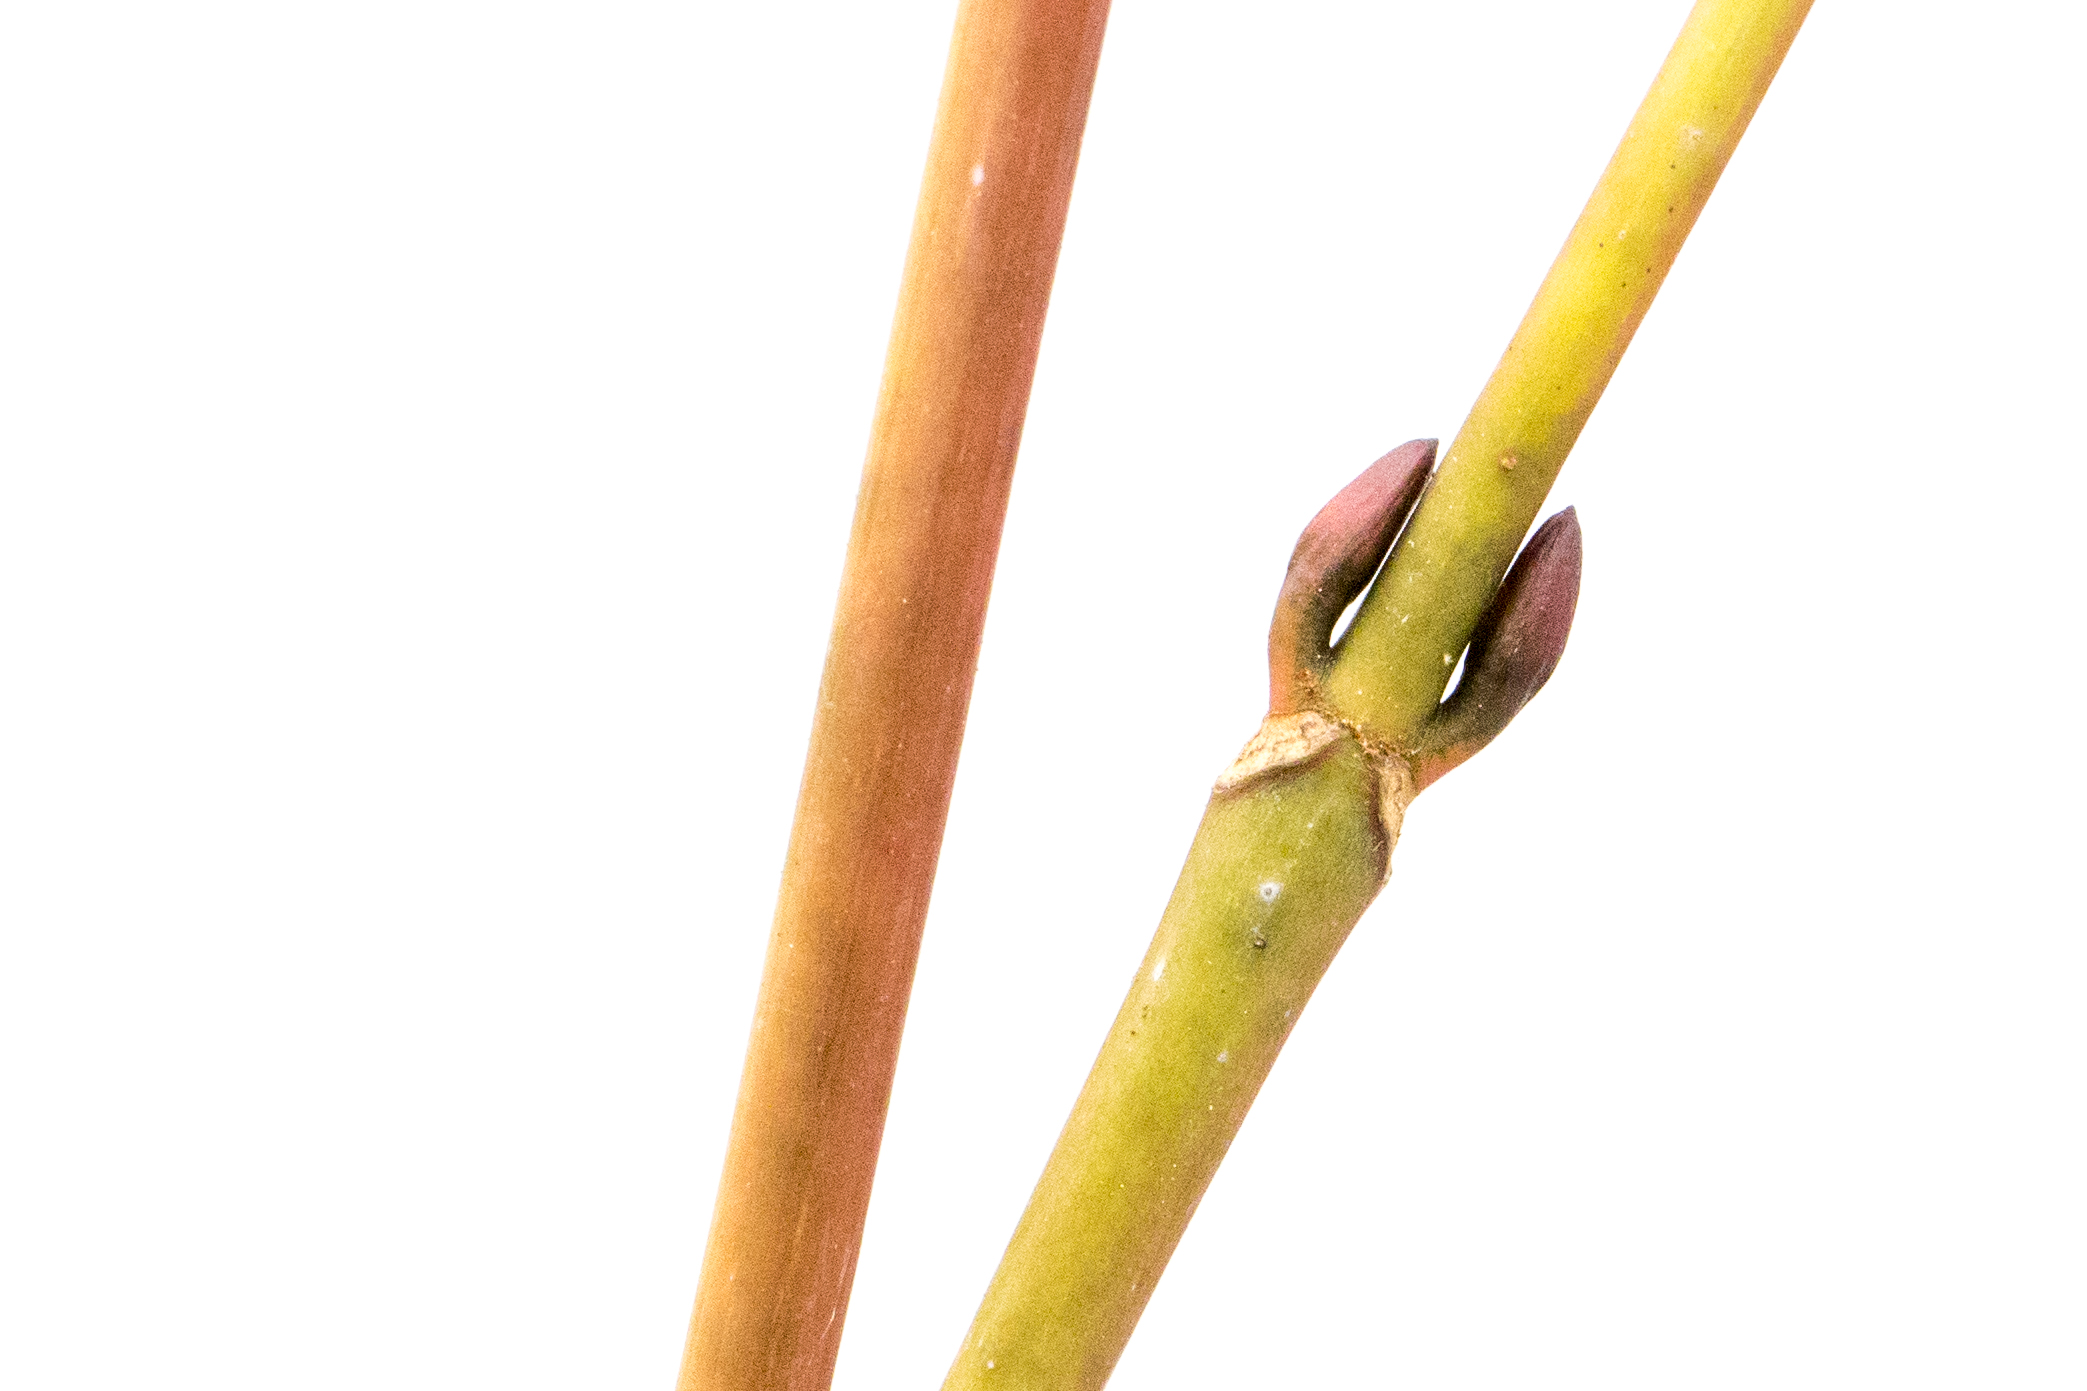
\includegraphics[width = 7cm]{acepen/Acer_pensylvanicum,_stage_00.jpg}}
              \hfill \subfigure[Stage 1]{
                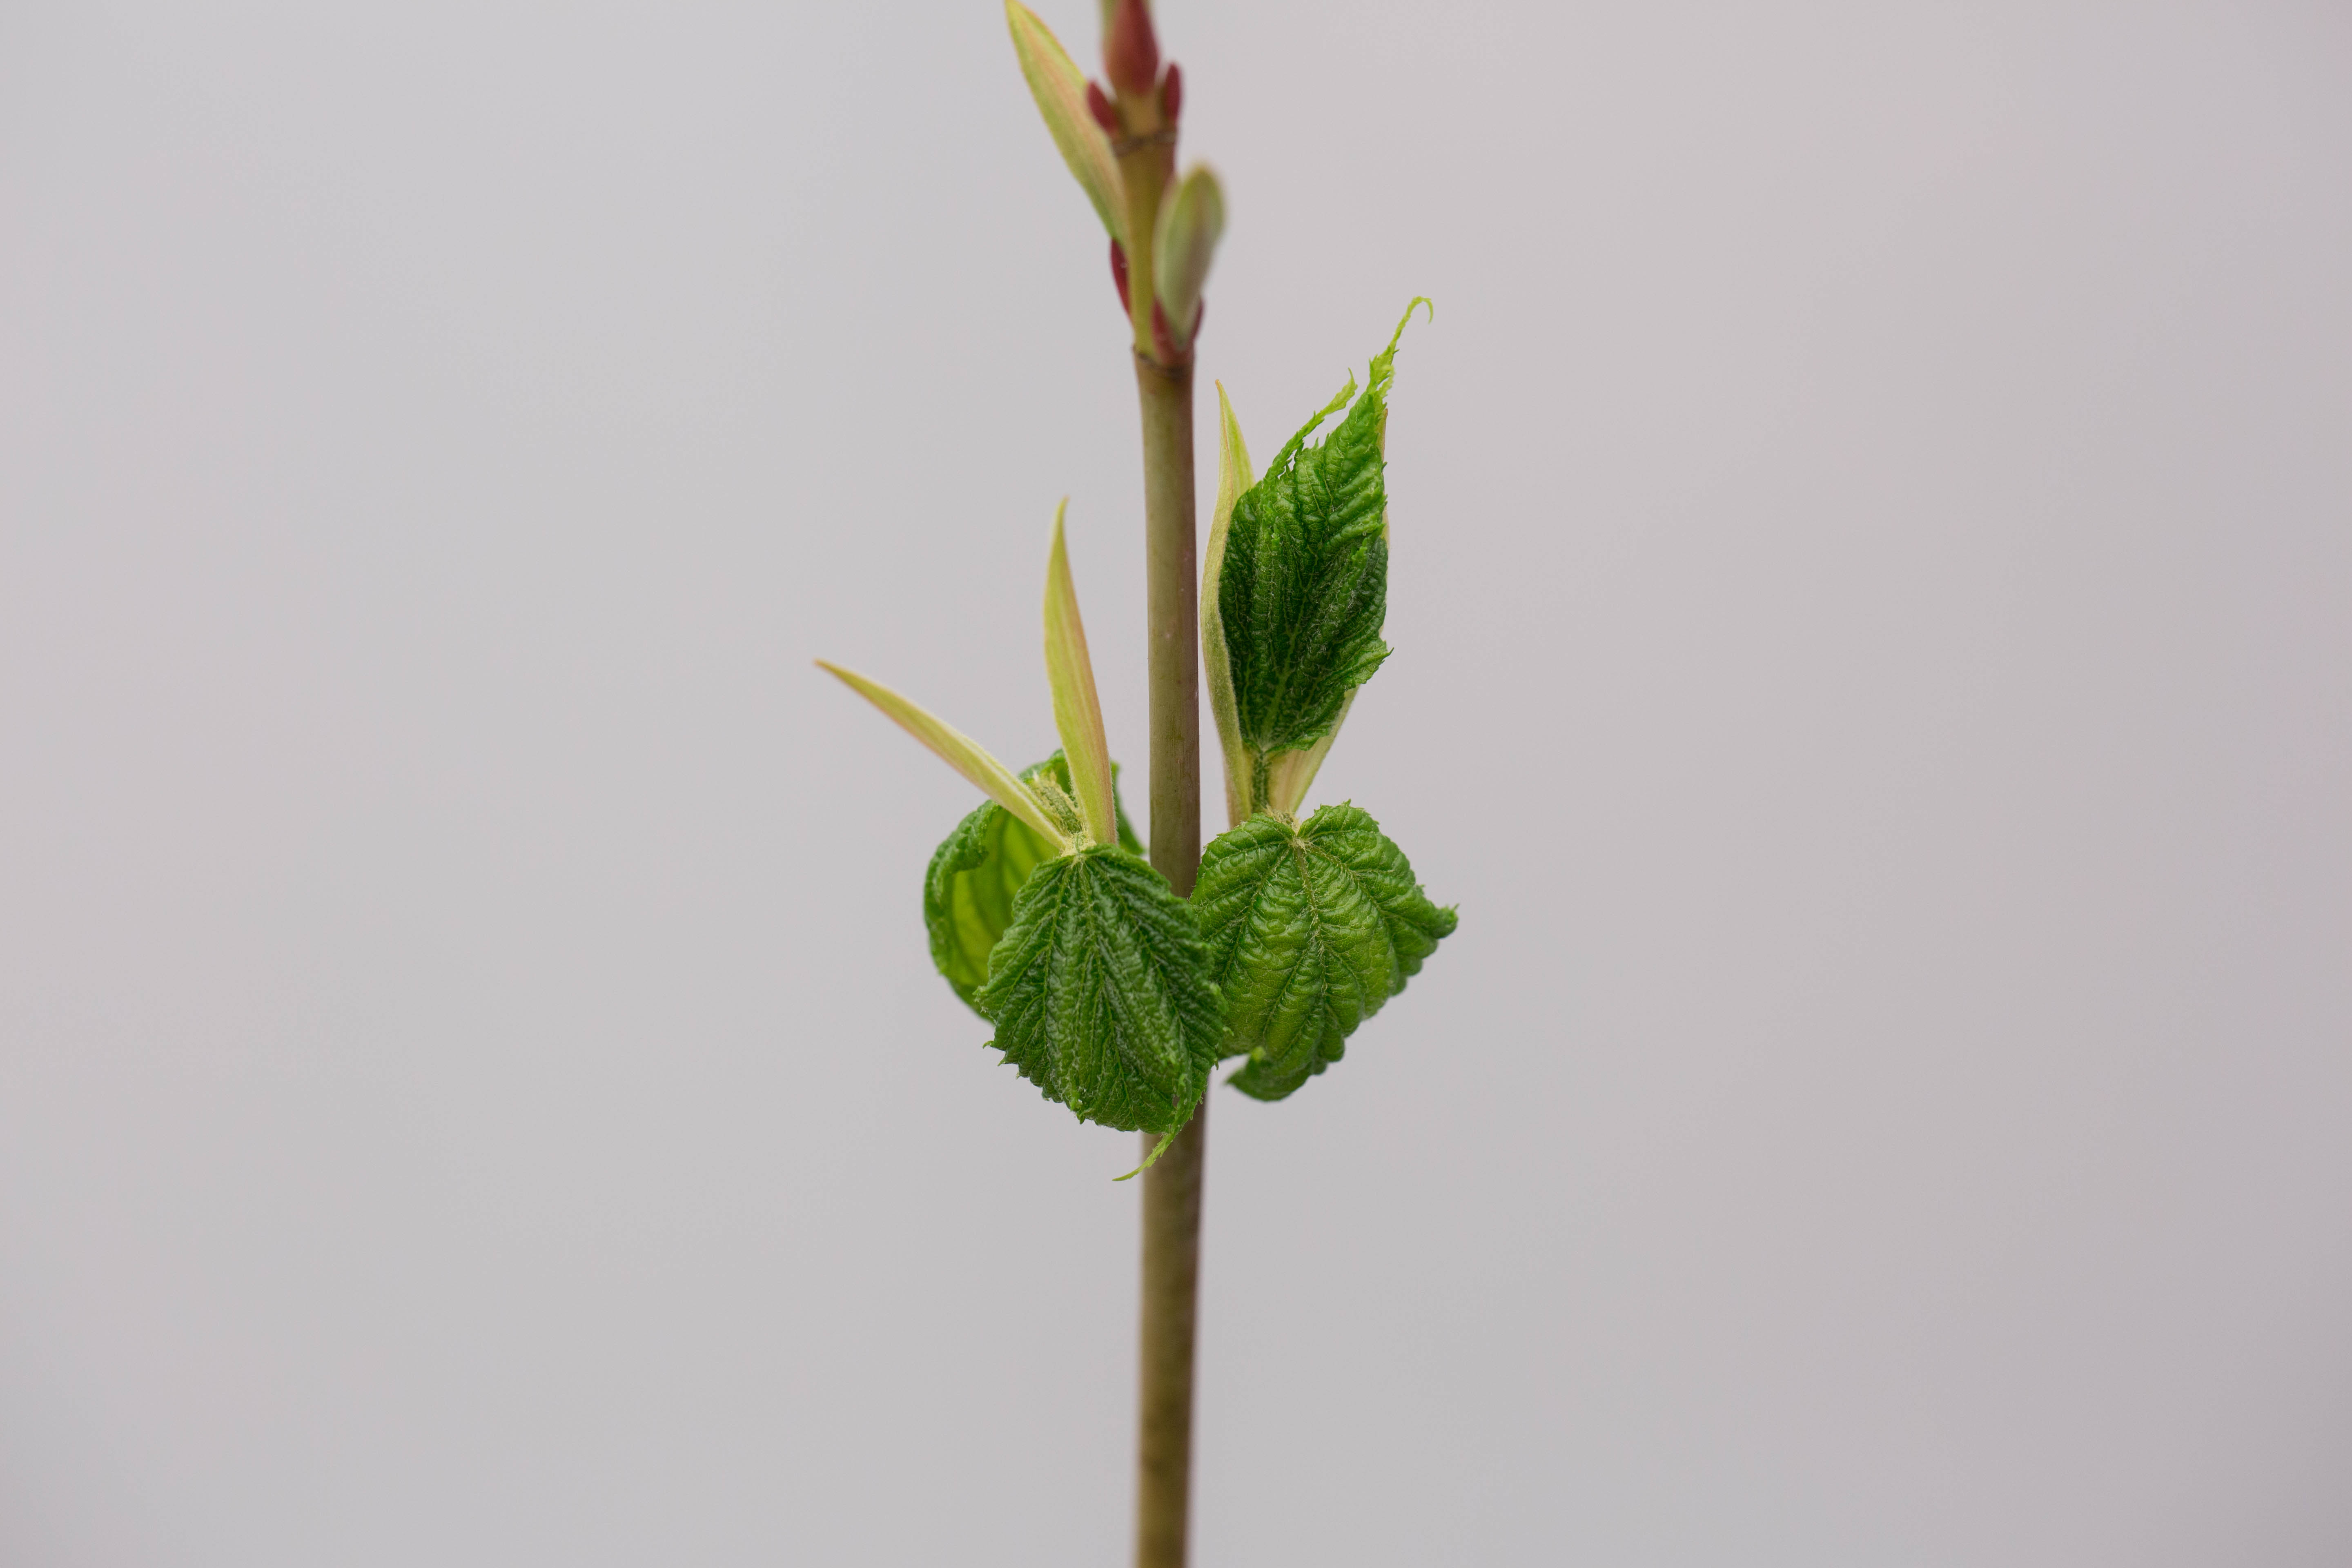
\includegraphics[width = 7cm]{acepen/Acer_pensylvanicum,_stage_01.jpg}}
              \hfill \subfigure[Stage 2]{
                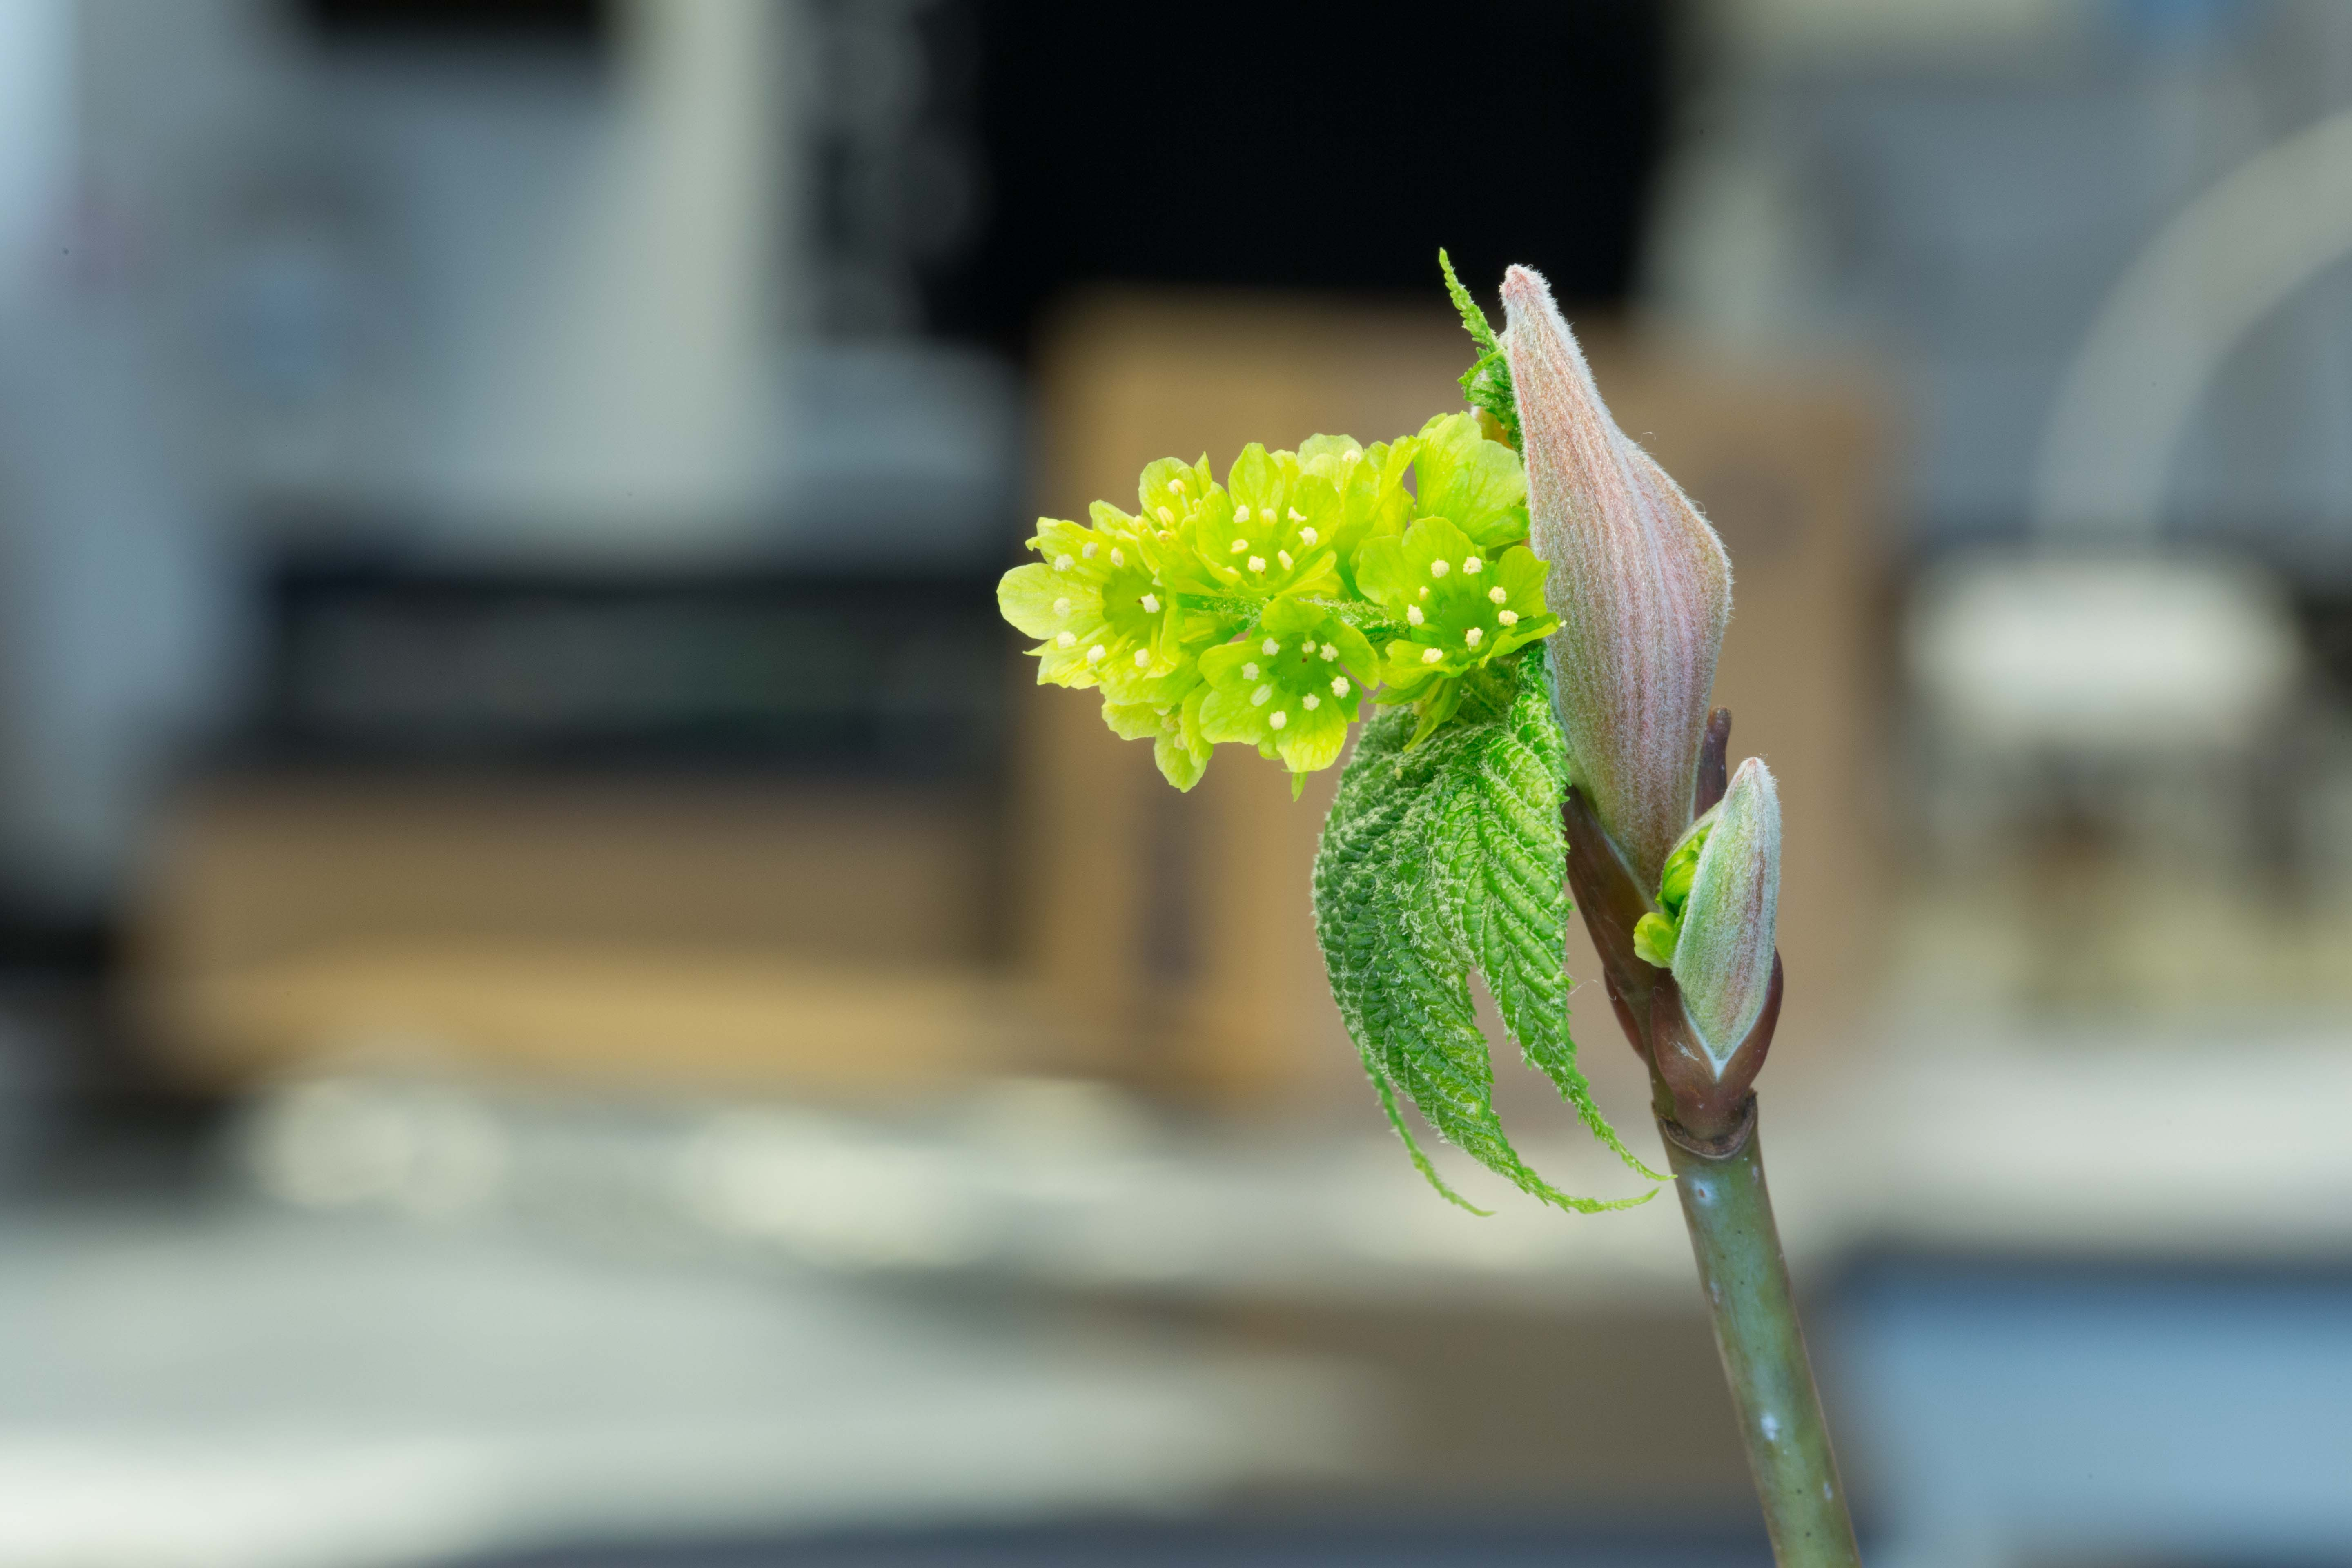
\includegraphics[width = 7cm]{acepen/Acer_pensylvanicum,_stage_02.jpg}}
              \hfill \subfigure[Stage 3]{
                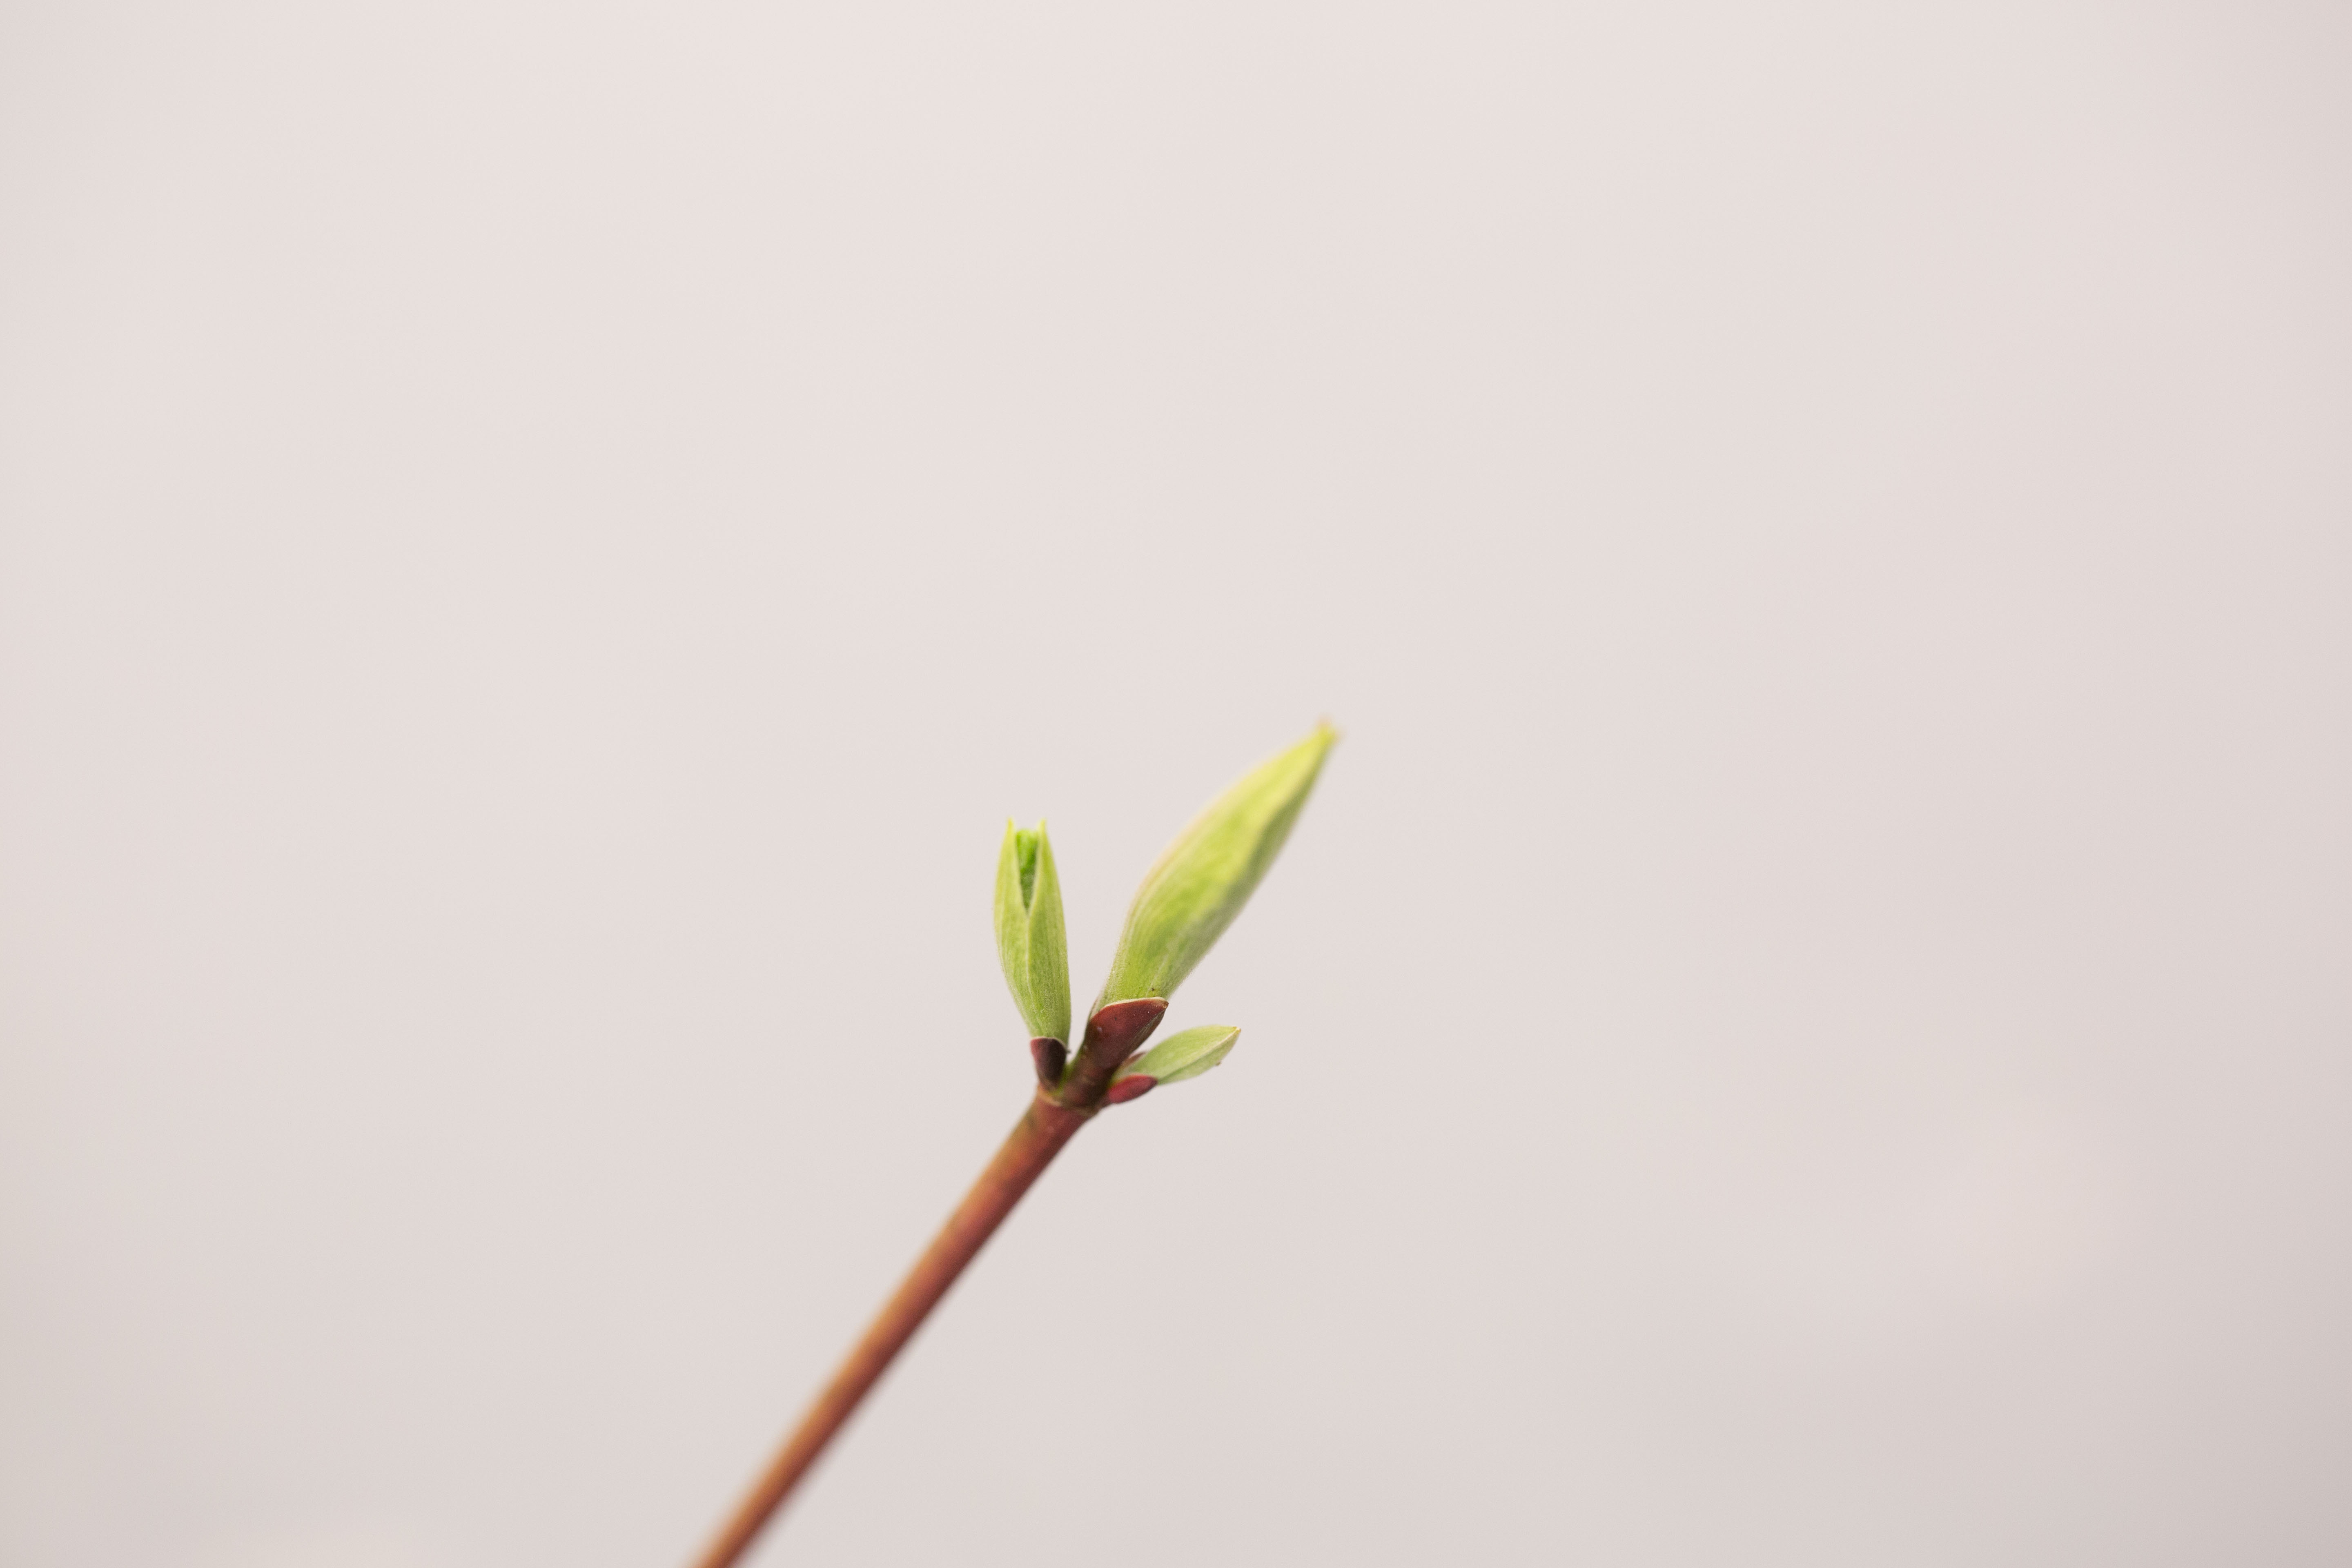
\includegraphics[width = 7cm]{acepen/Acer_pensylvanicum,_stage_03.jpg}}
              \hfill \subfigure[Stage 4]{
                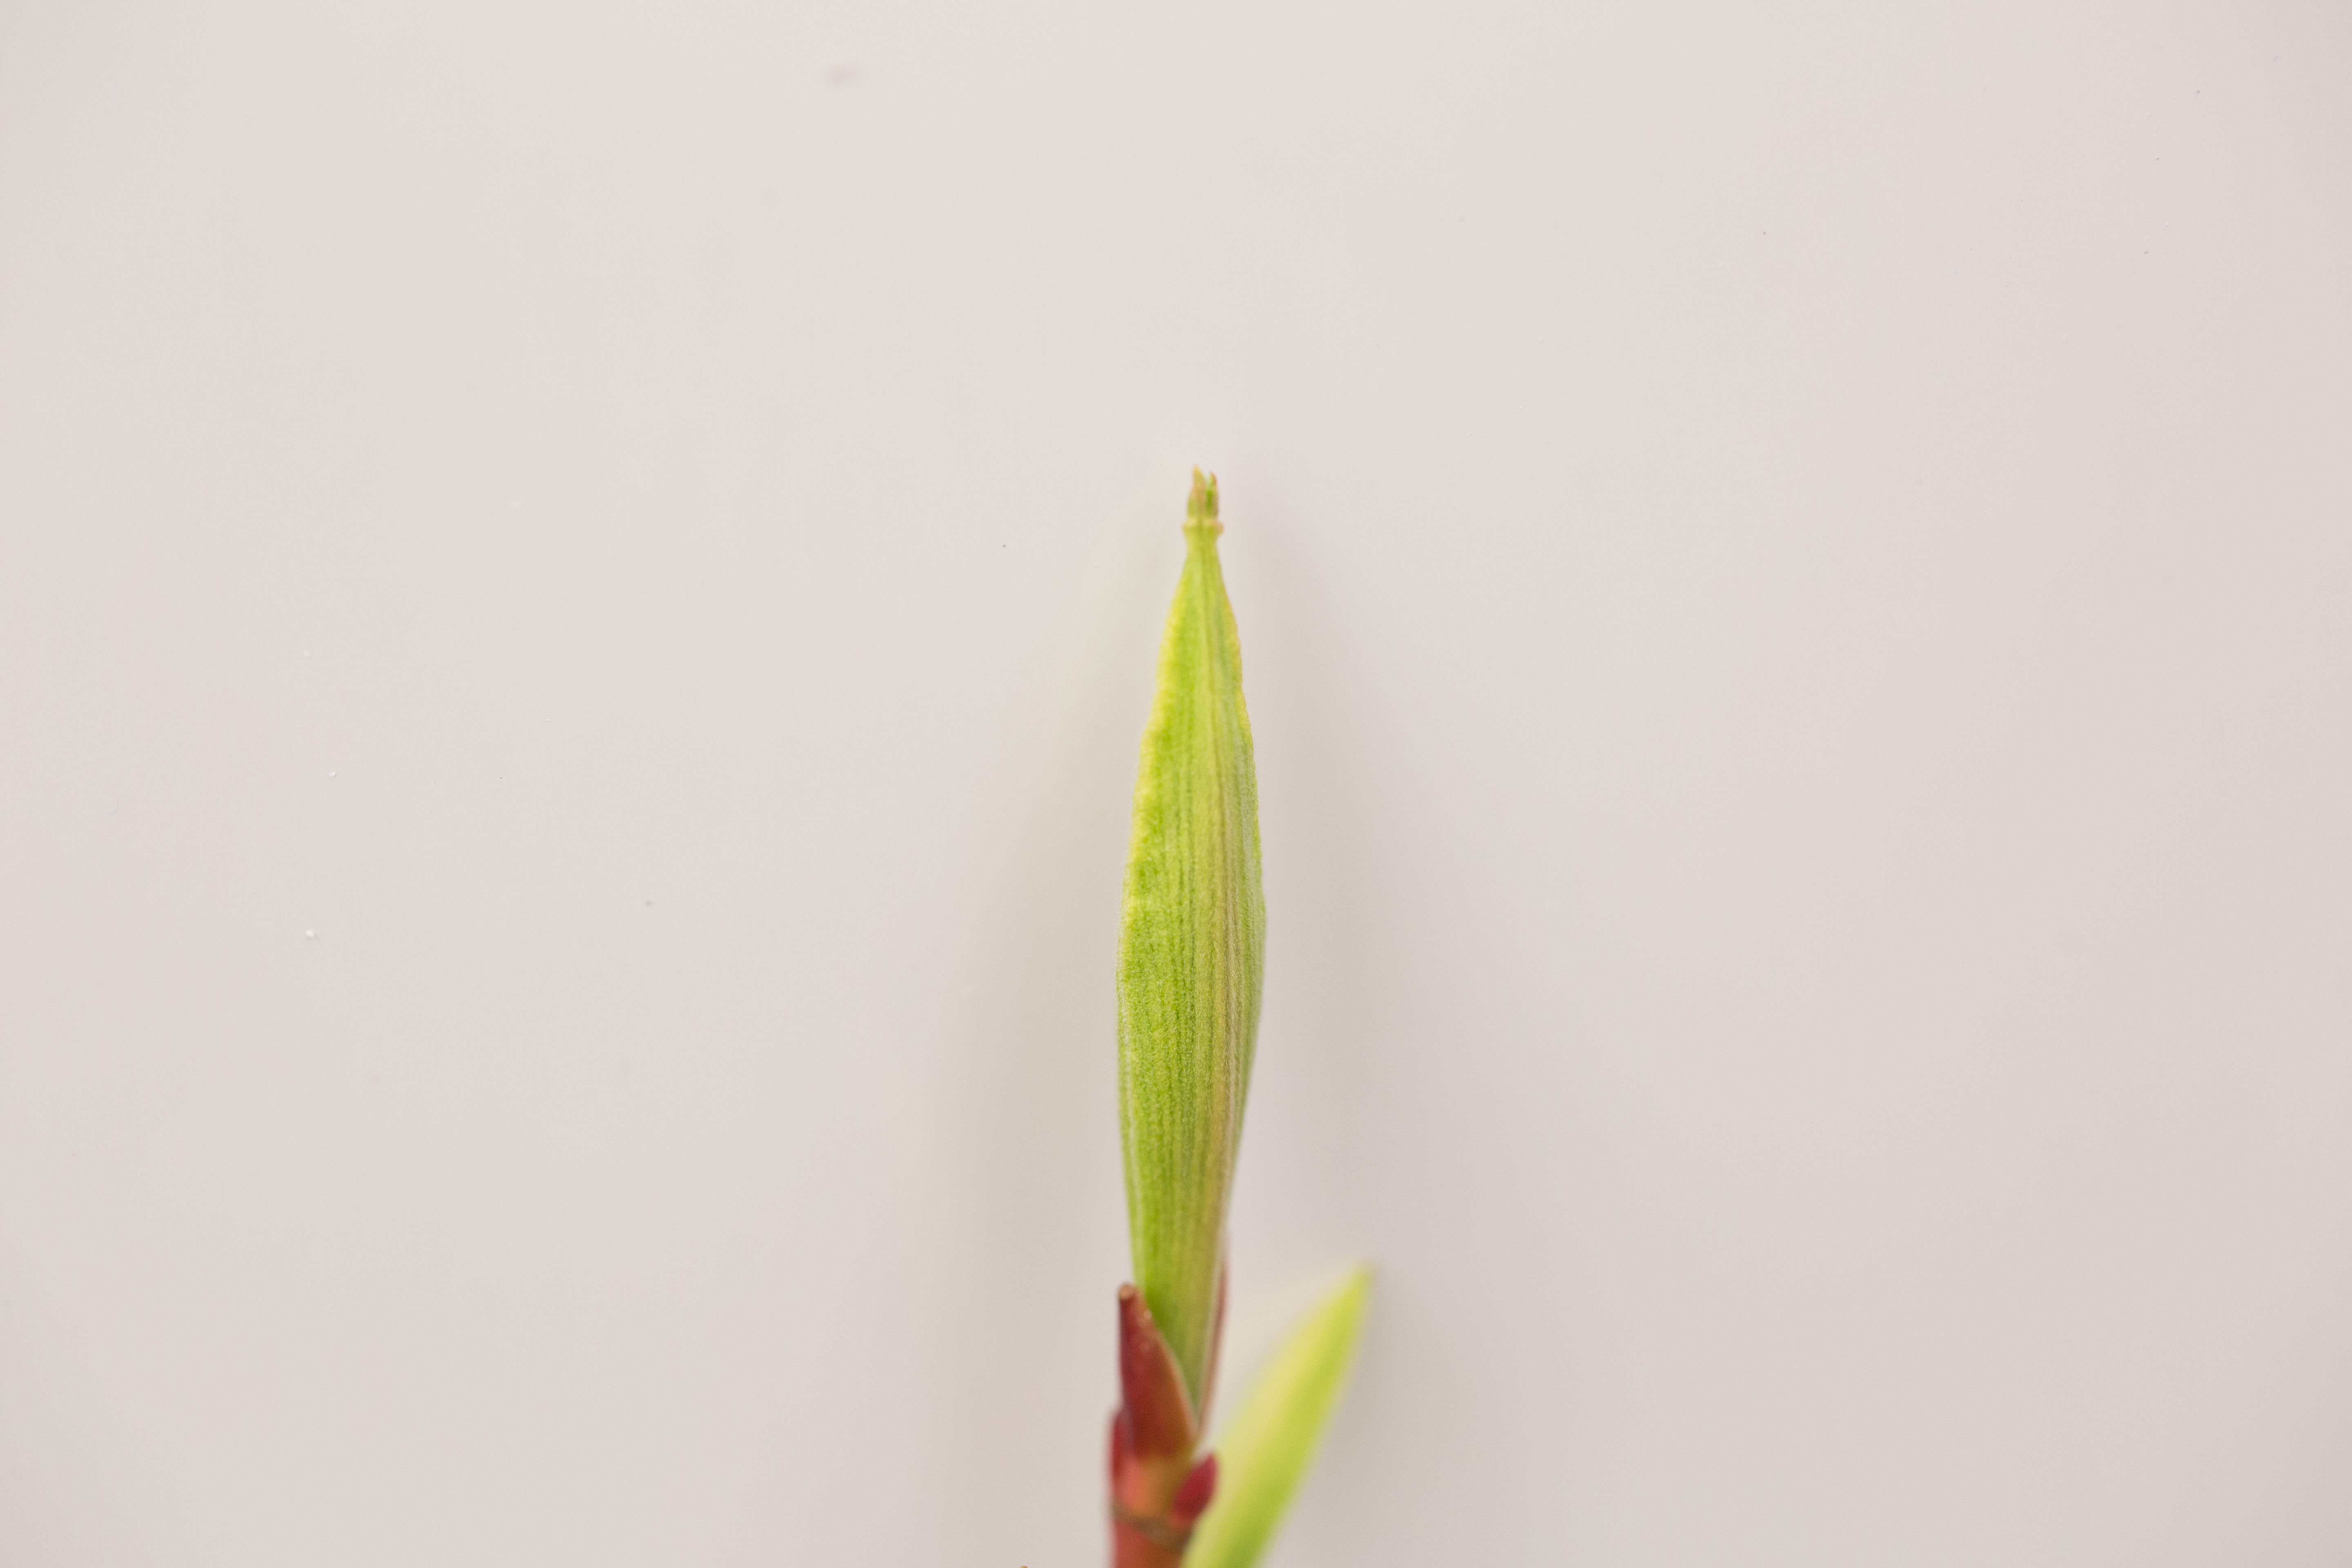
\includegraphics[width = 7cm]{acepen/Acer_pensylvanicum,_stage_04.jpg}}
              \hfill \subfigure[Stage 5]{
                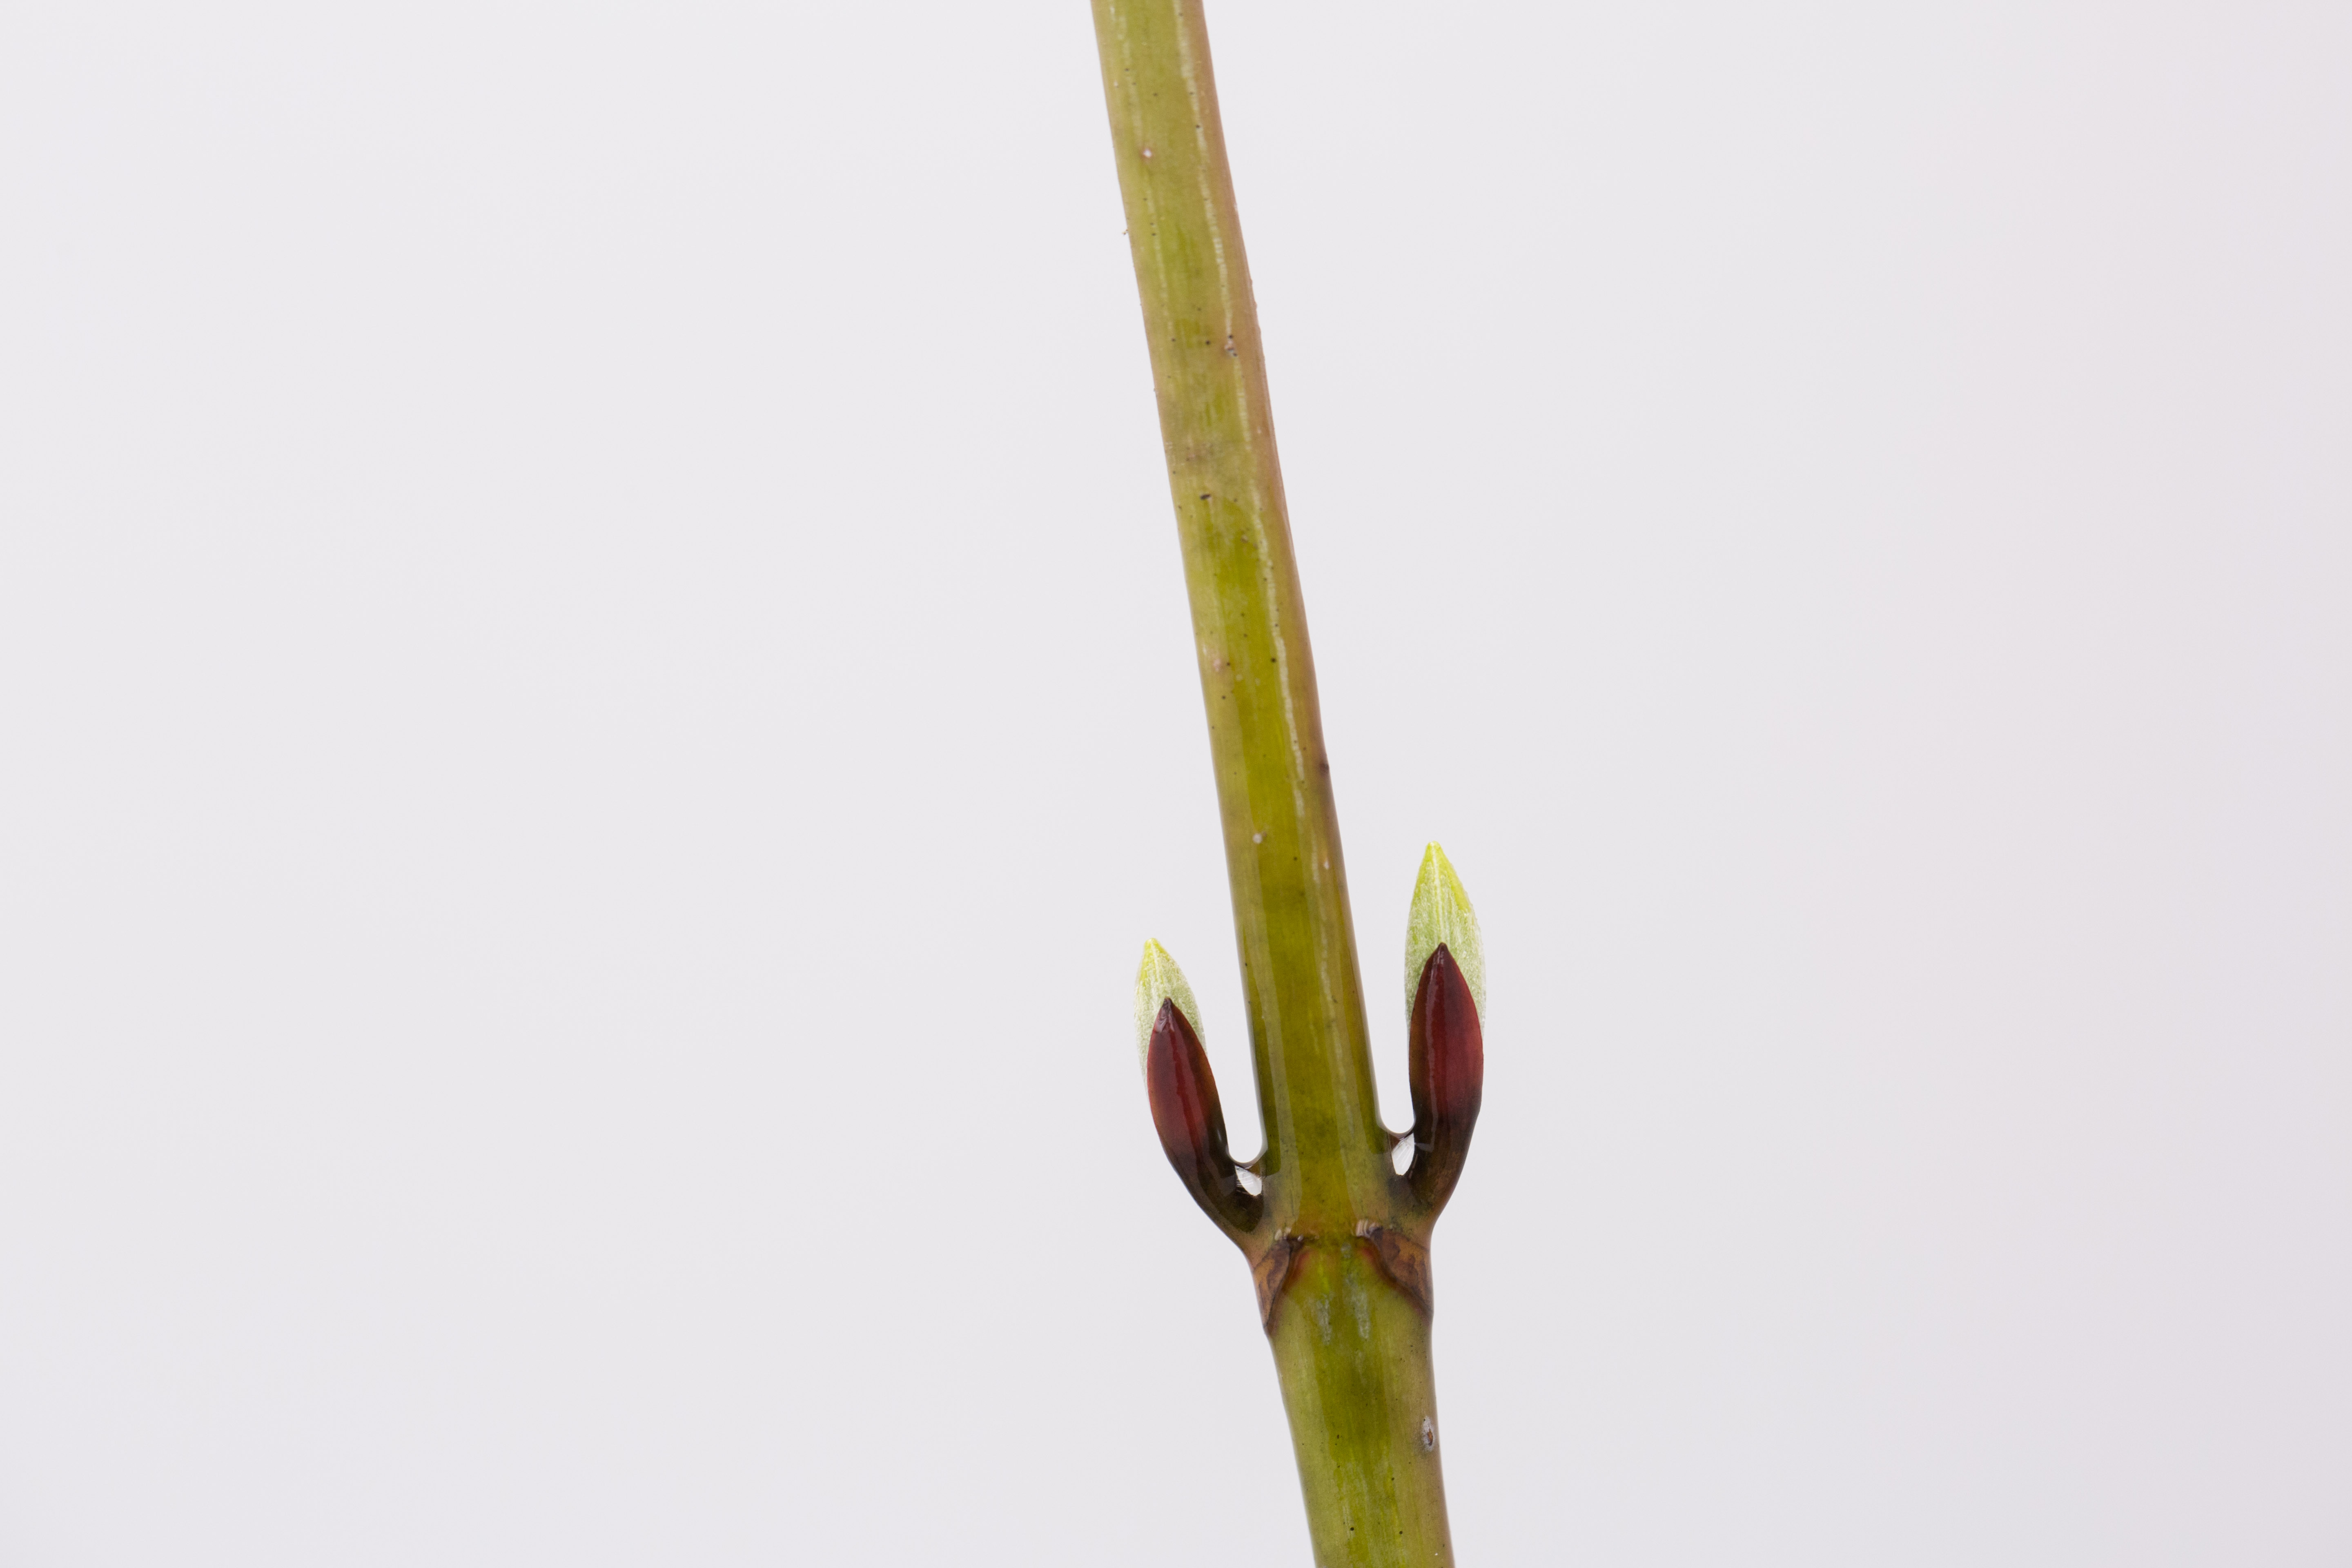
\includegraphics[width = 7cm]{acepen/Acer_pensylvanicum,_stage_05.jpg}}
              \hfill \caption{\textit{Acer pensylvanicum}}\end{figure}\newpage
\begin{figure}[ht]\centering\hfill \subfigure[Stage 0]{
                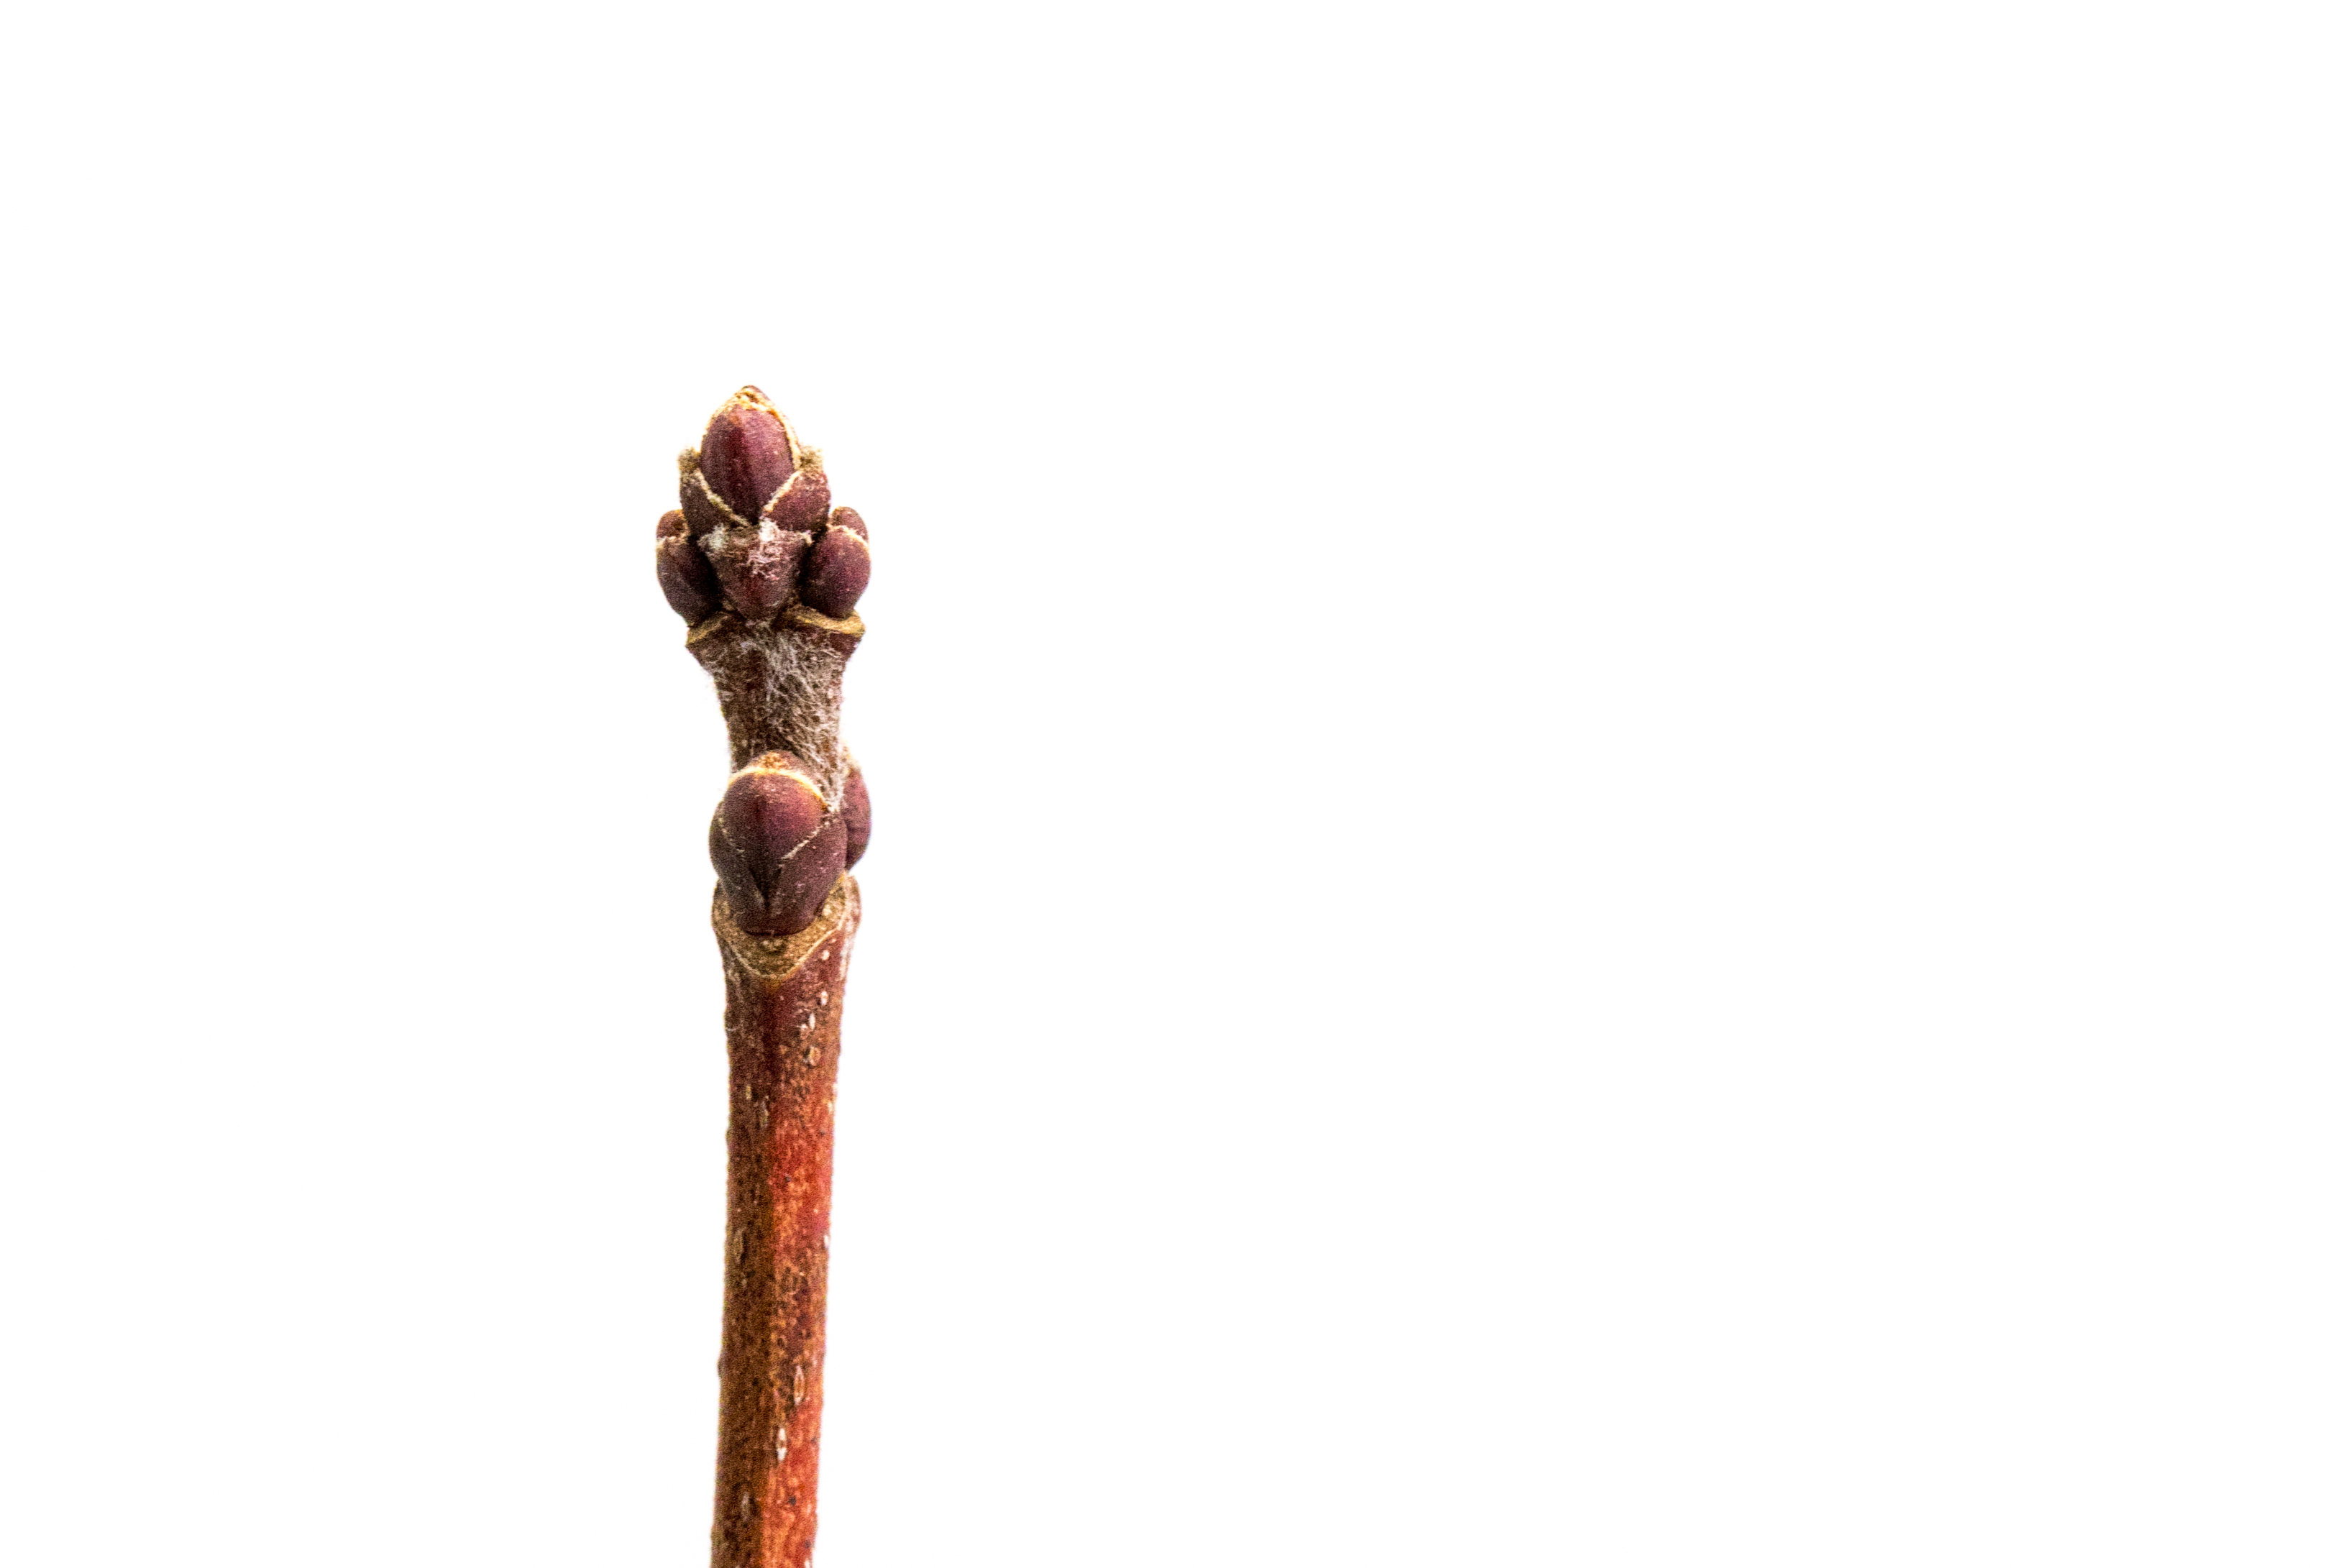
\includegraphics[width = 7cm]{acerub/Acer_rubrum,_stage_00.jpg}}
              \hfill \subfigure[Stage 1]{
                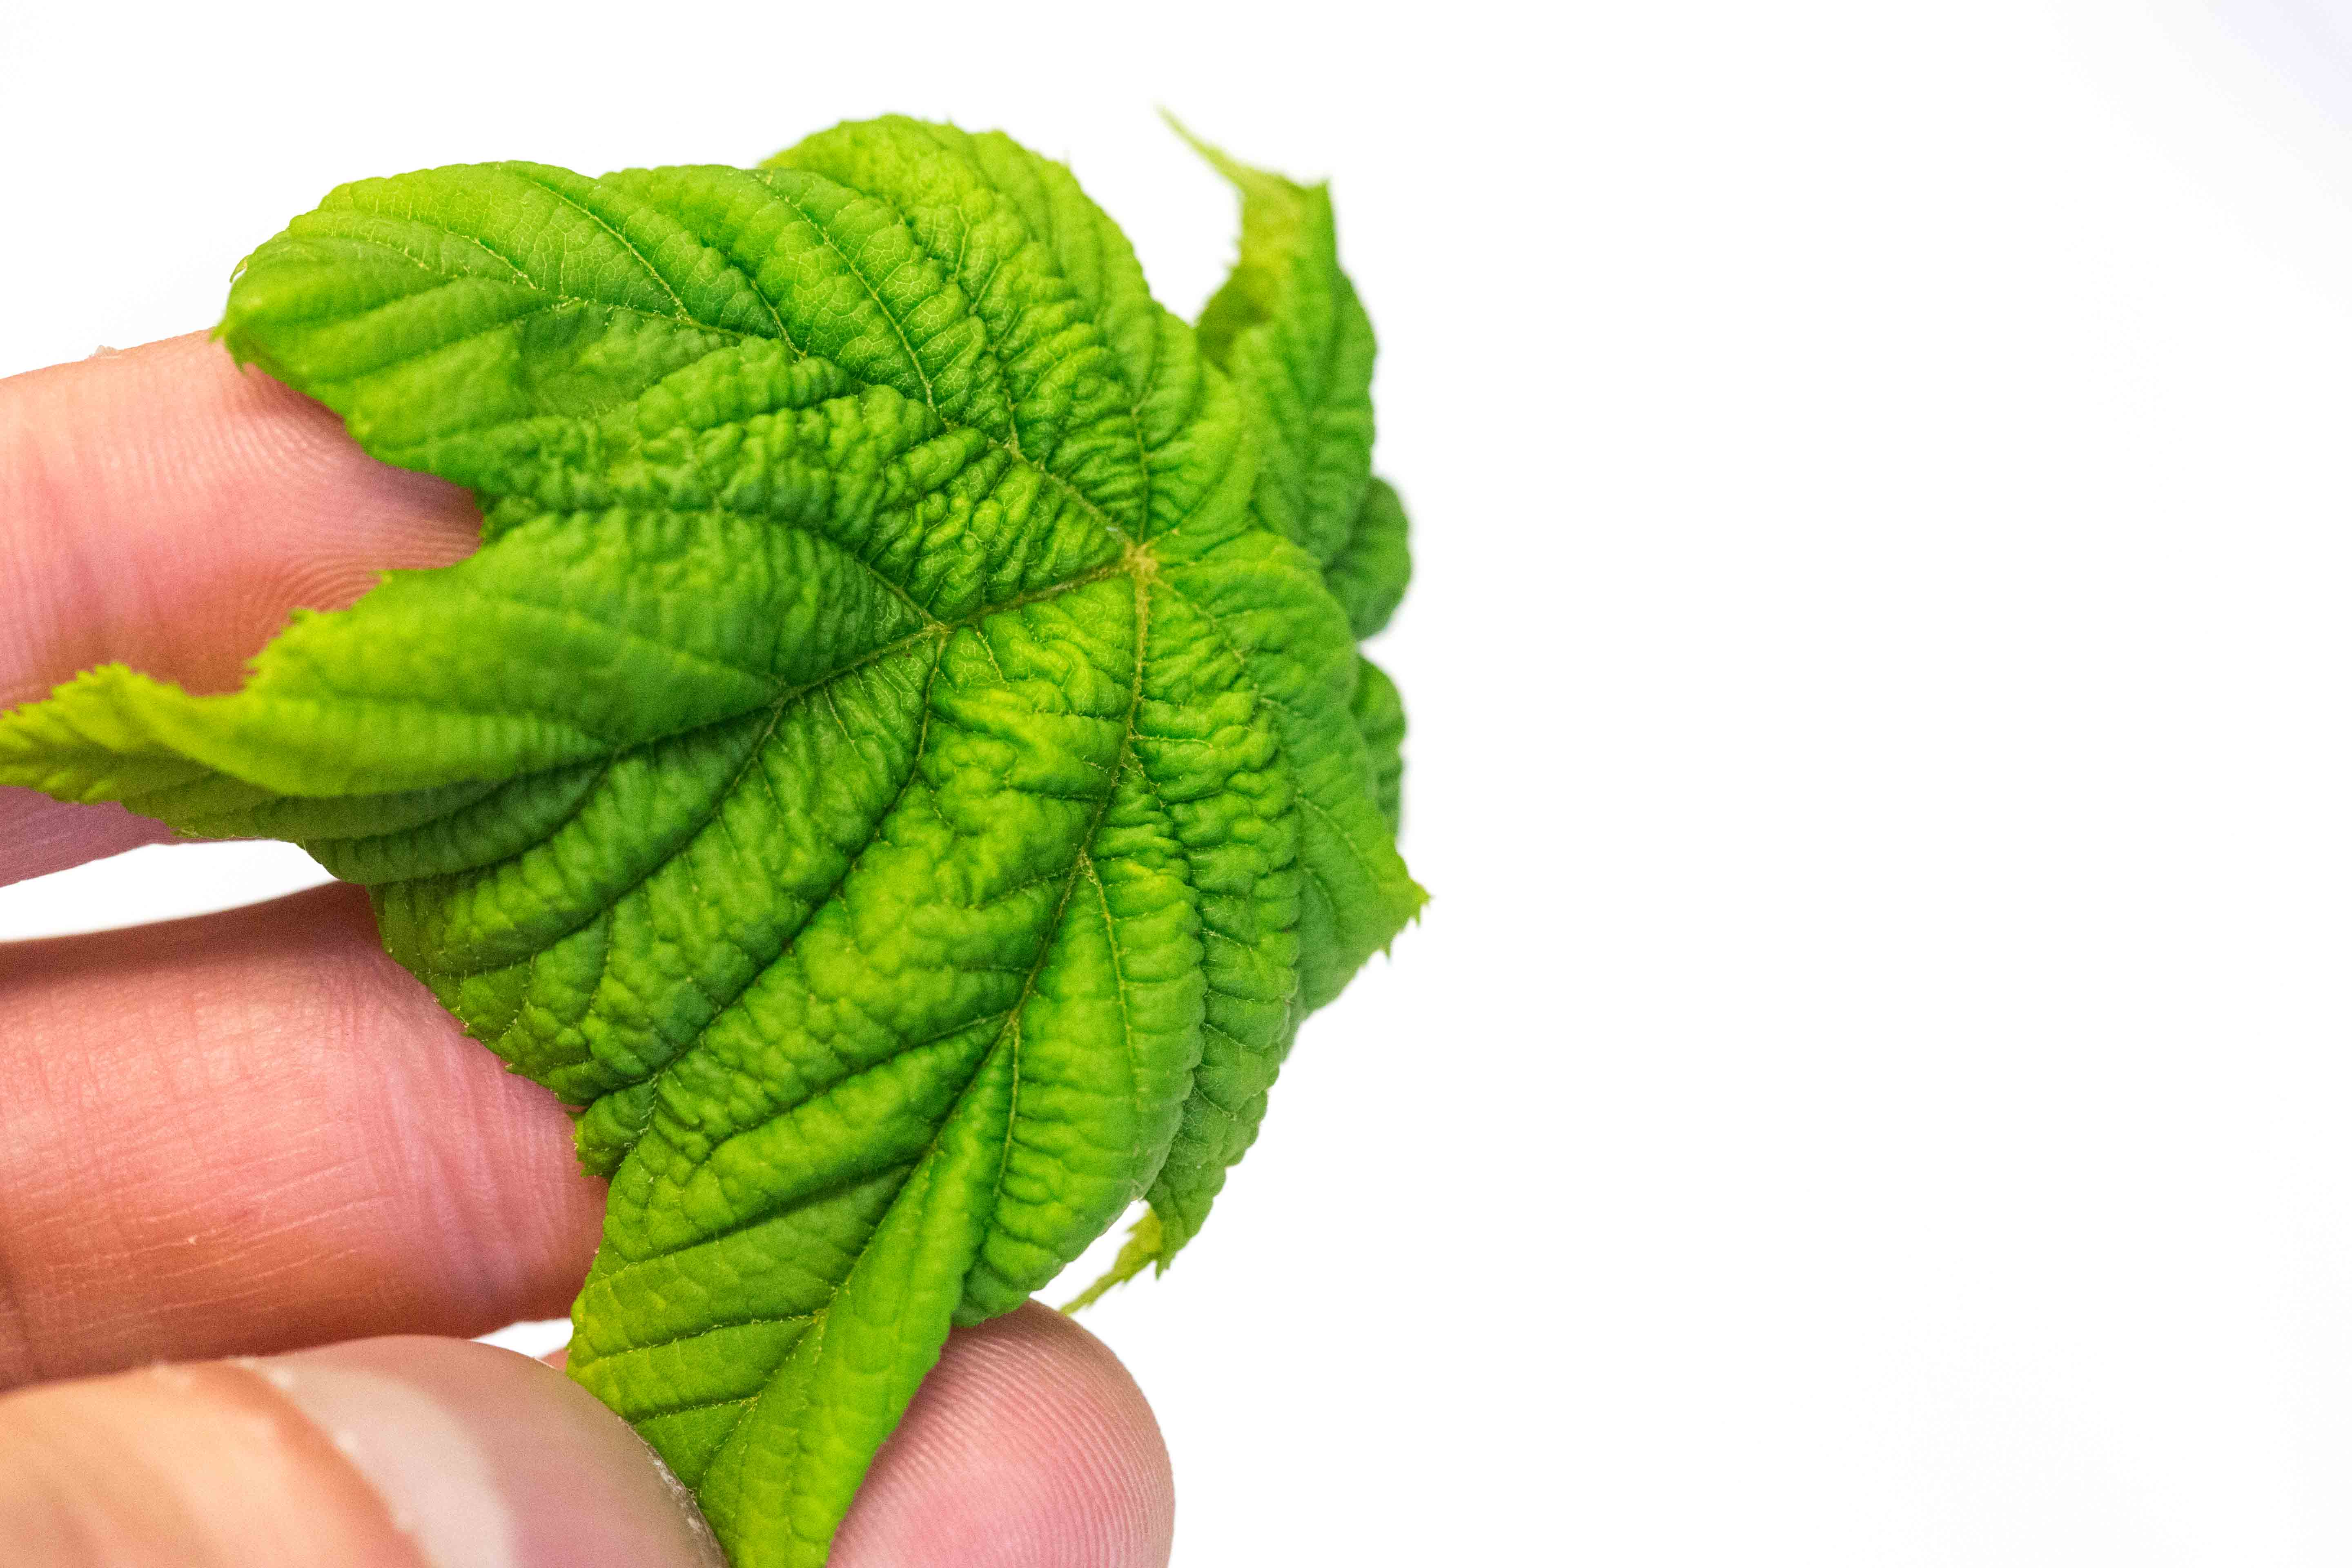
\includegraphics[width = 7cm]{acerub/Acer_rubrum,_stage_01.jpg}}
              \hfill \subfigure[Stage 2]{
                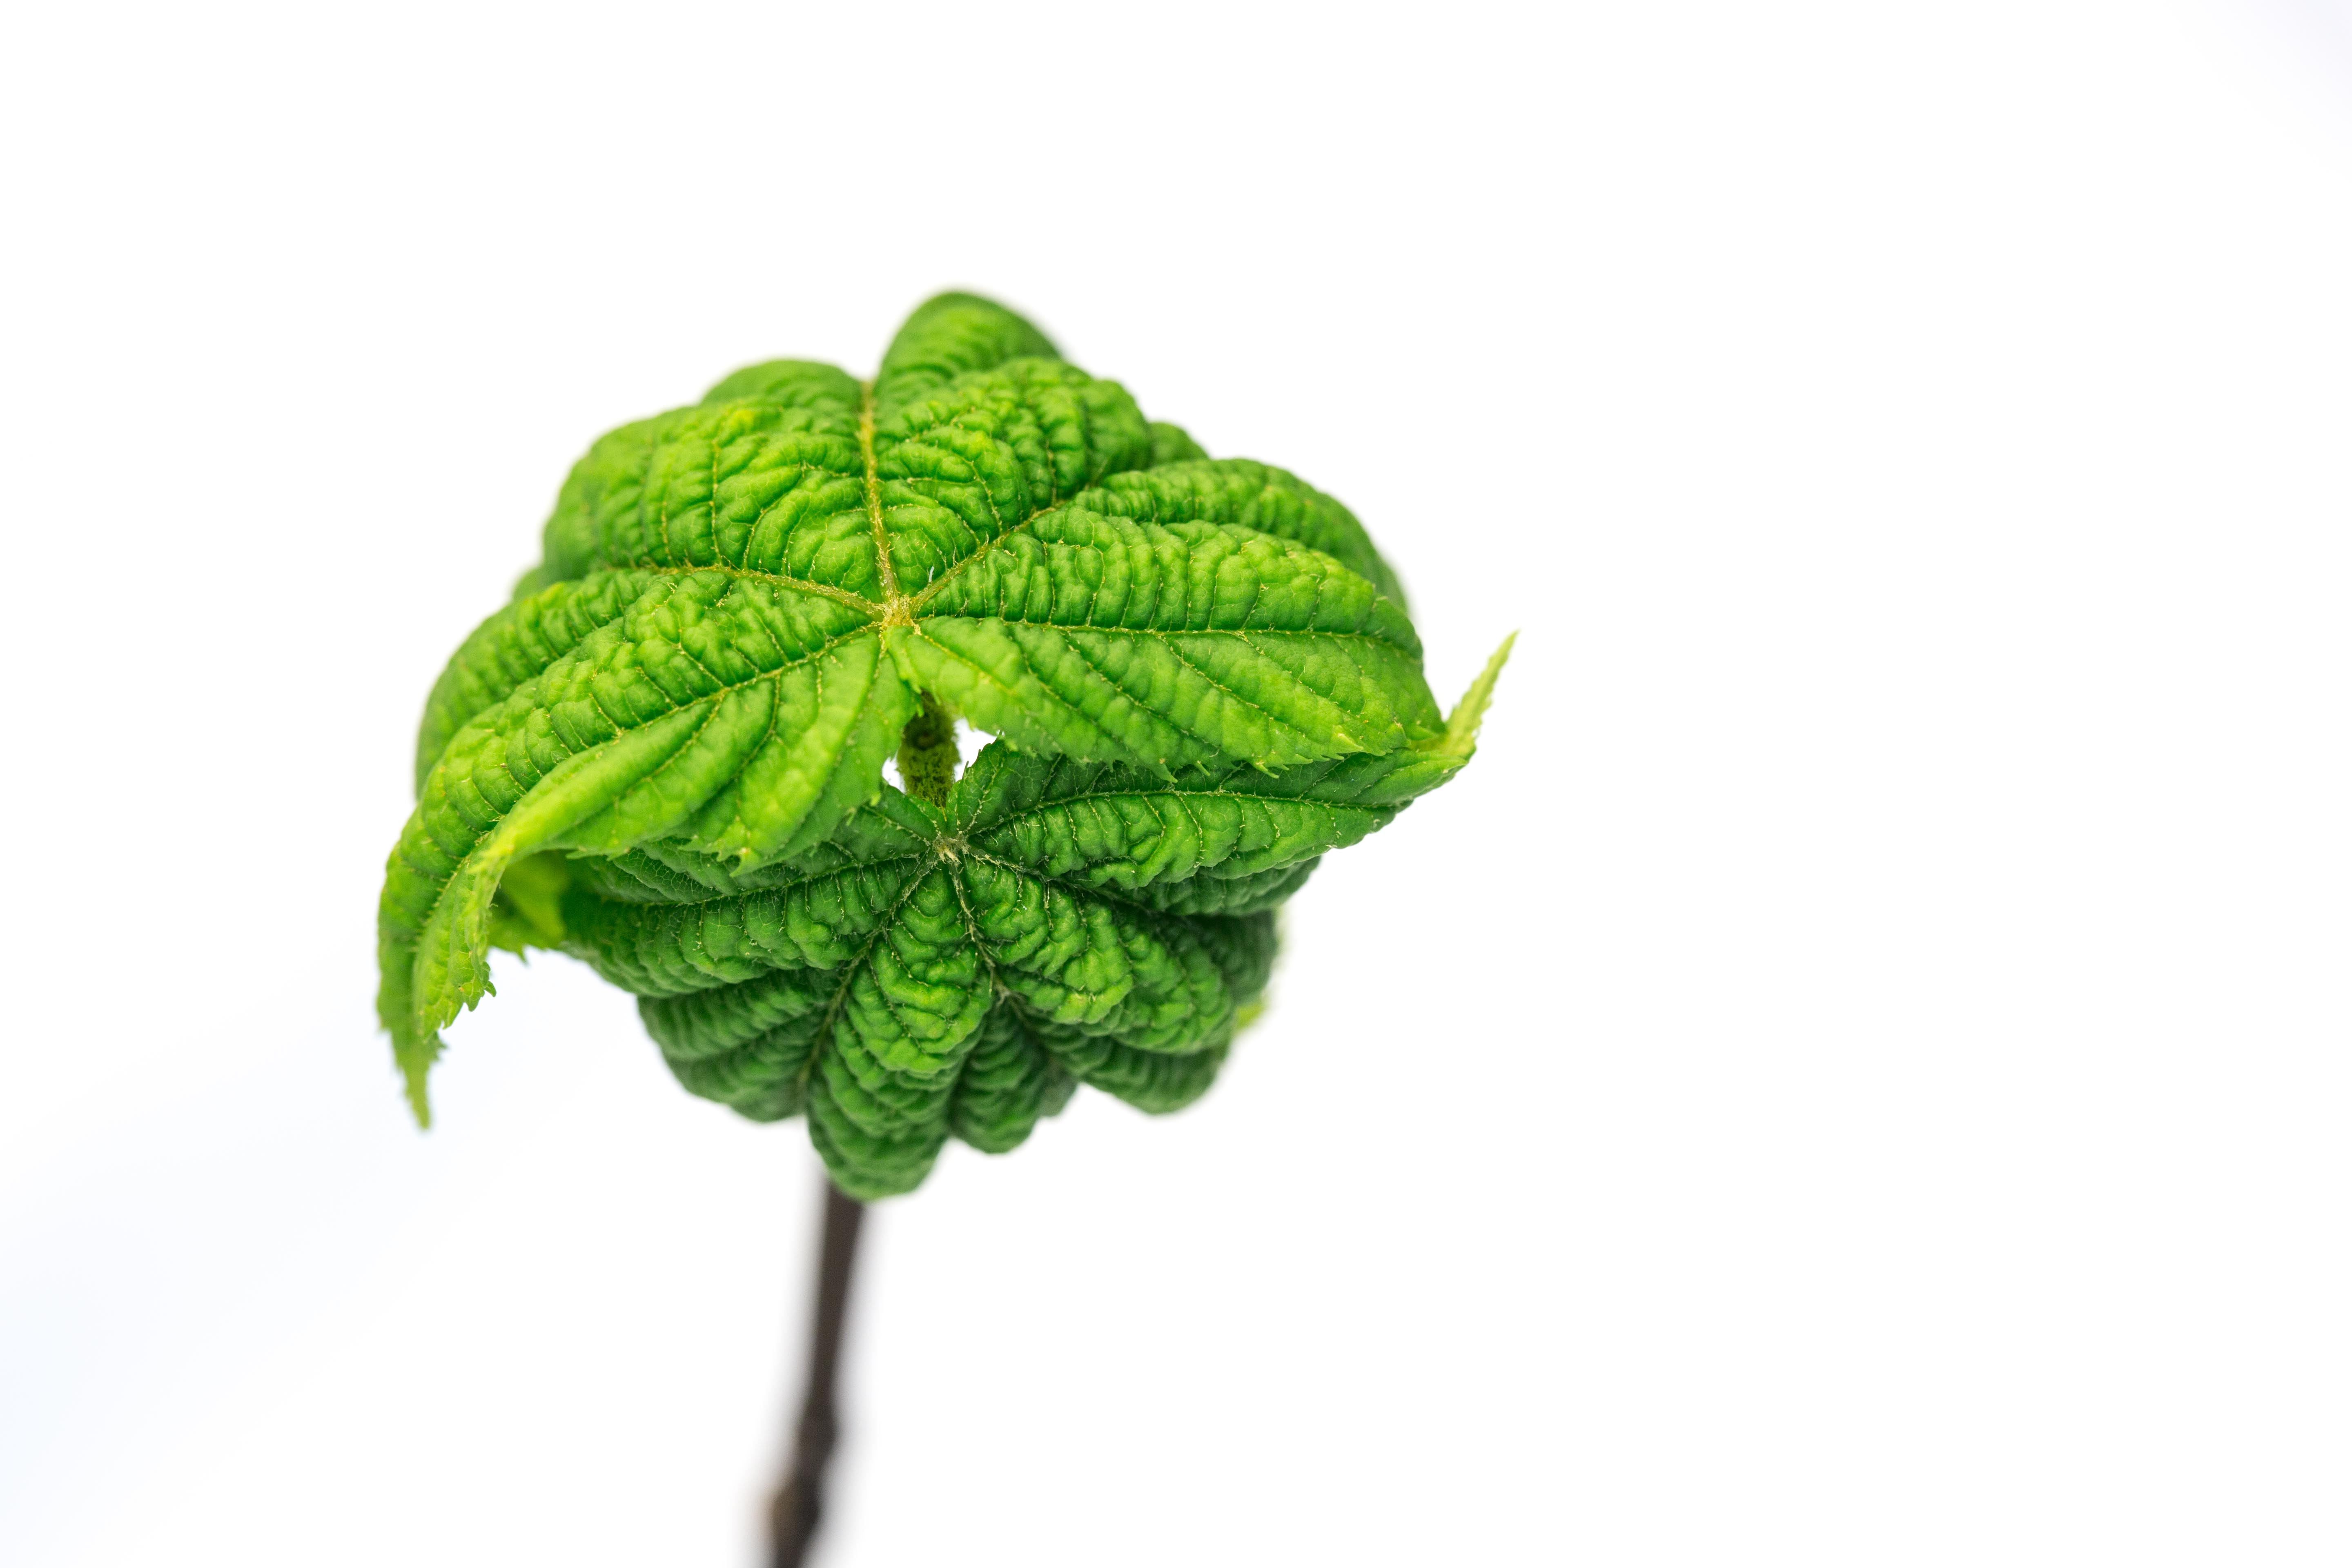
\includegraphics[width = 7cm]{acerub/Acer_rubrum,_stage_02.jpg}}
              \hfill \subfigure[Stage 3]{
                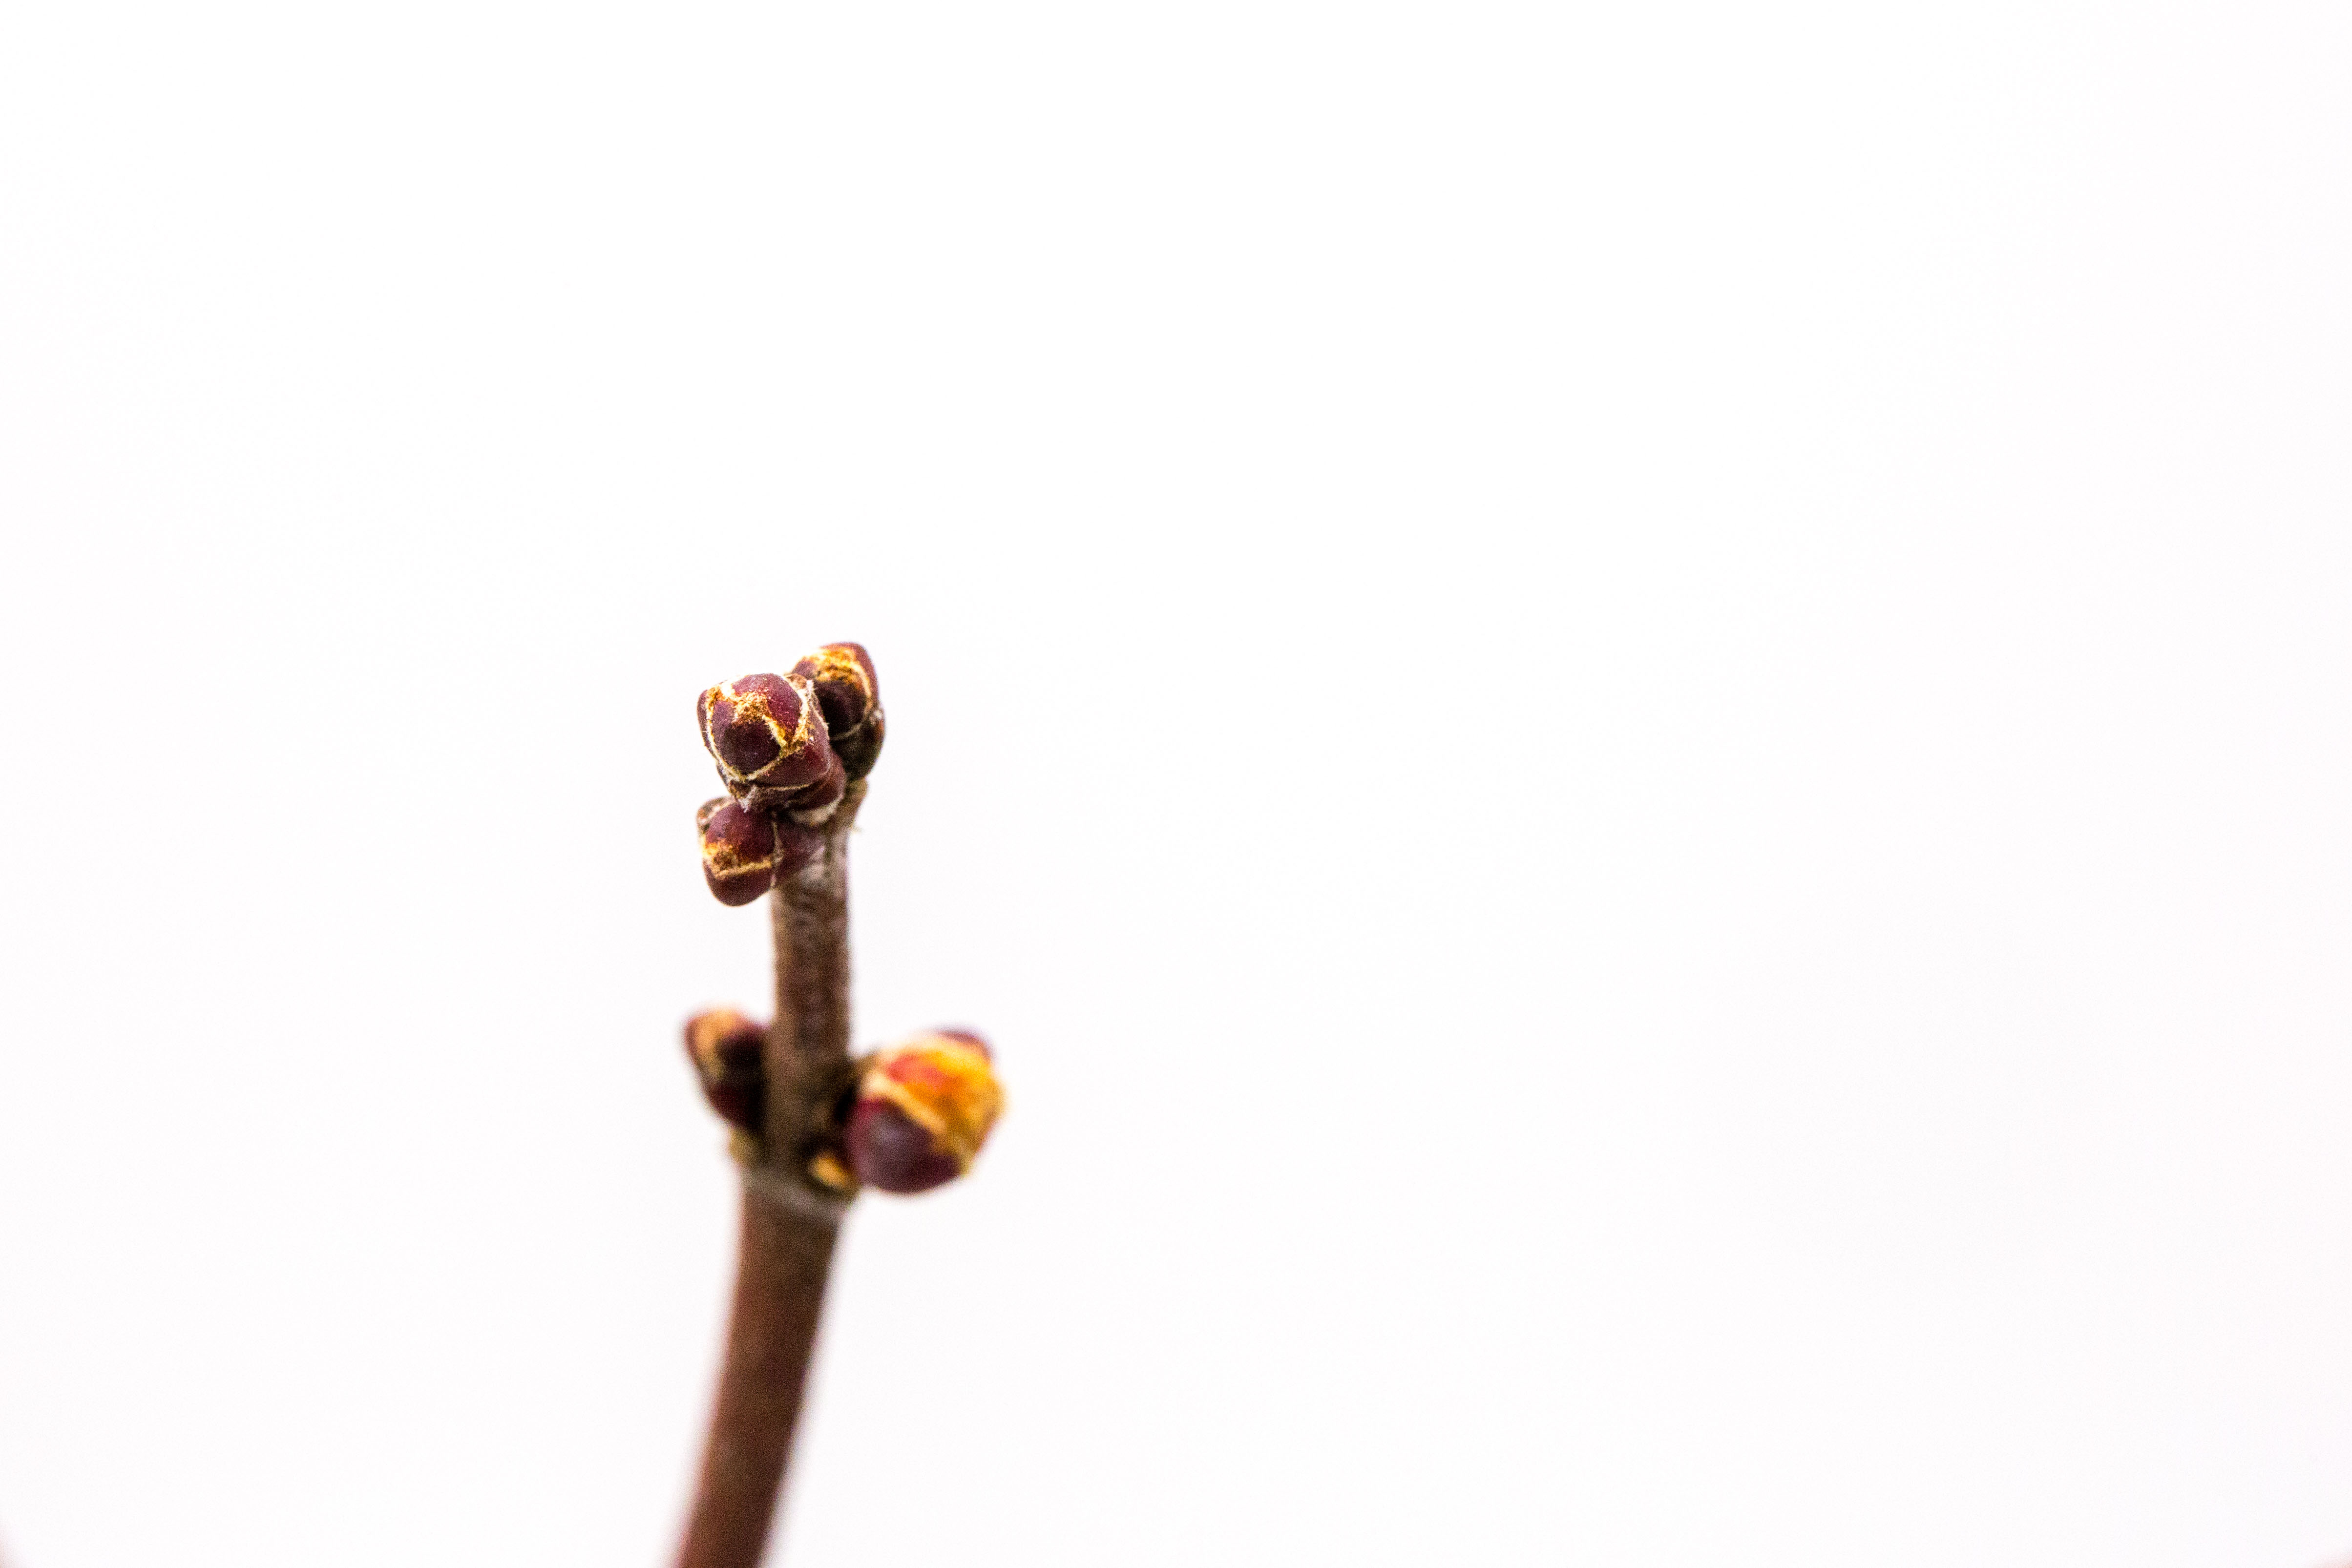
\includegraphics[width = 7cm]{acerub/Acer_rubrum,_stage_03.jpg}}
              \hfill \subfigure[Stage 4]{
                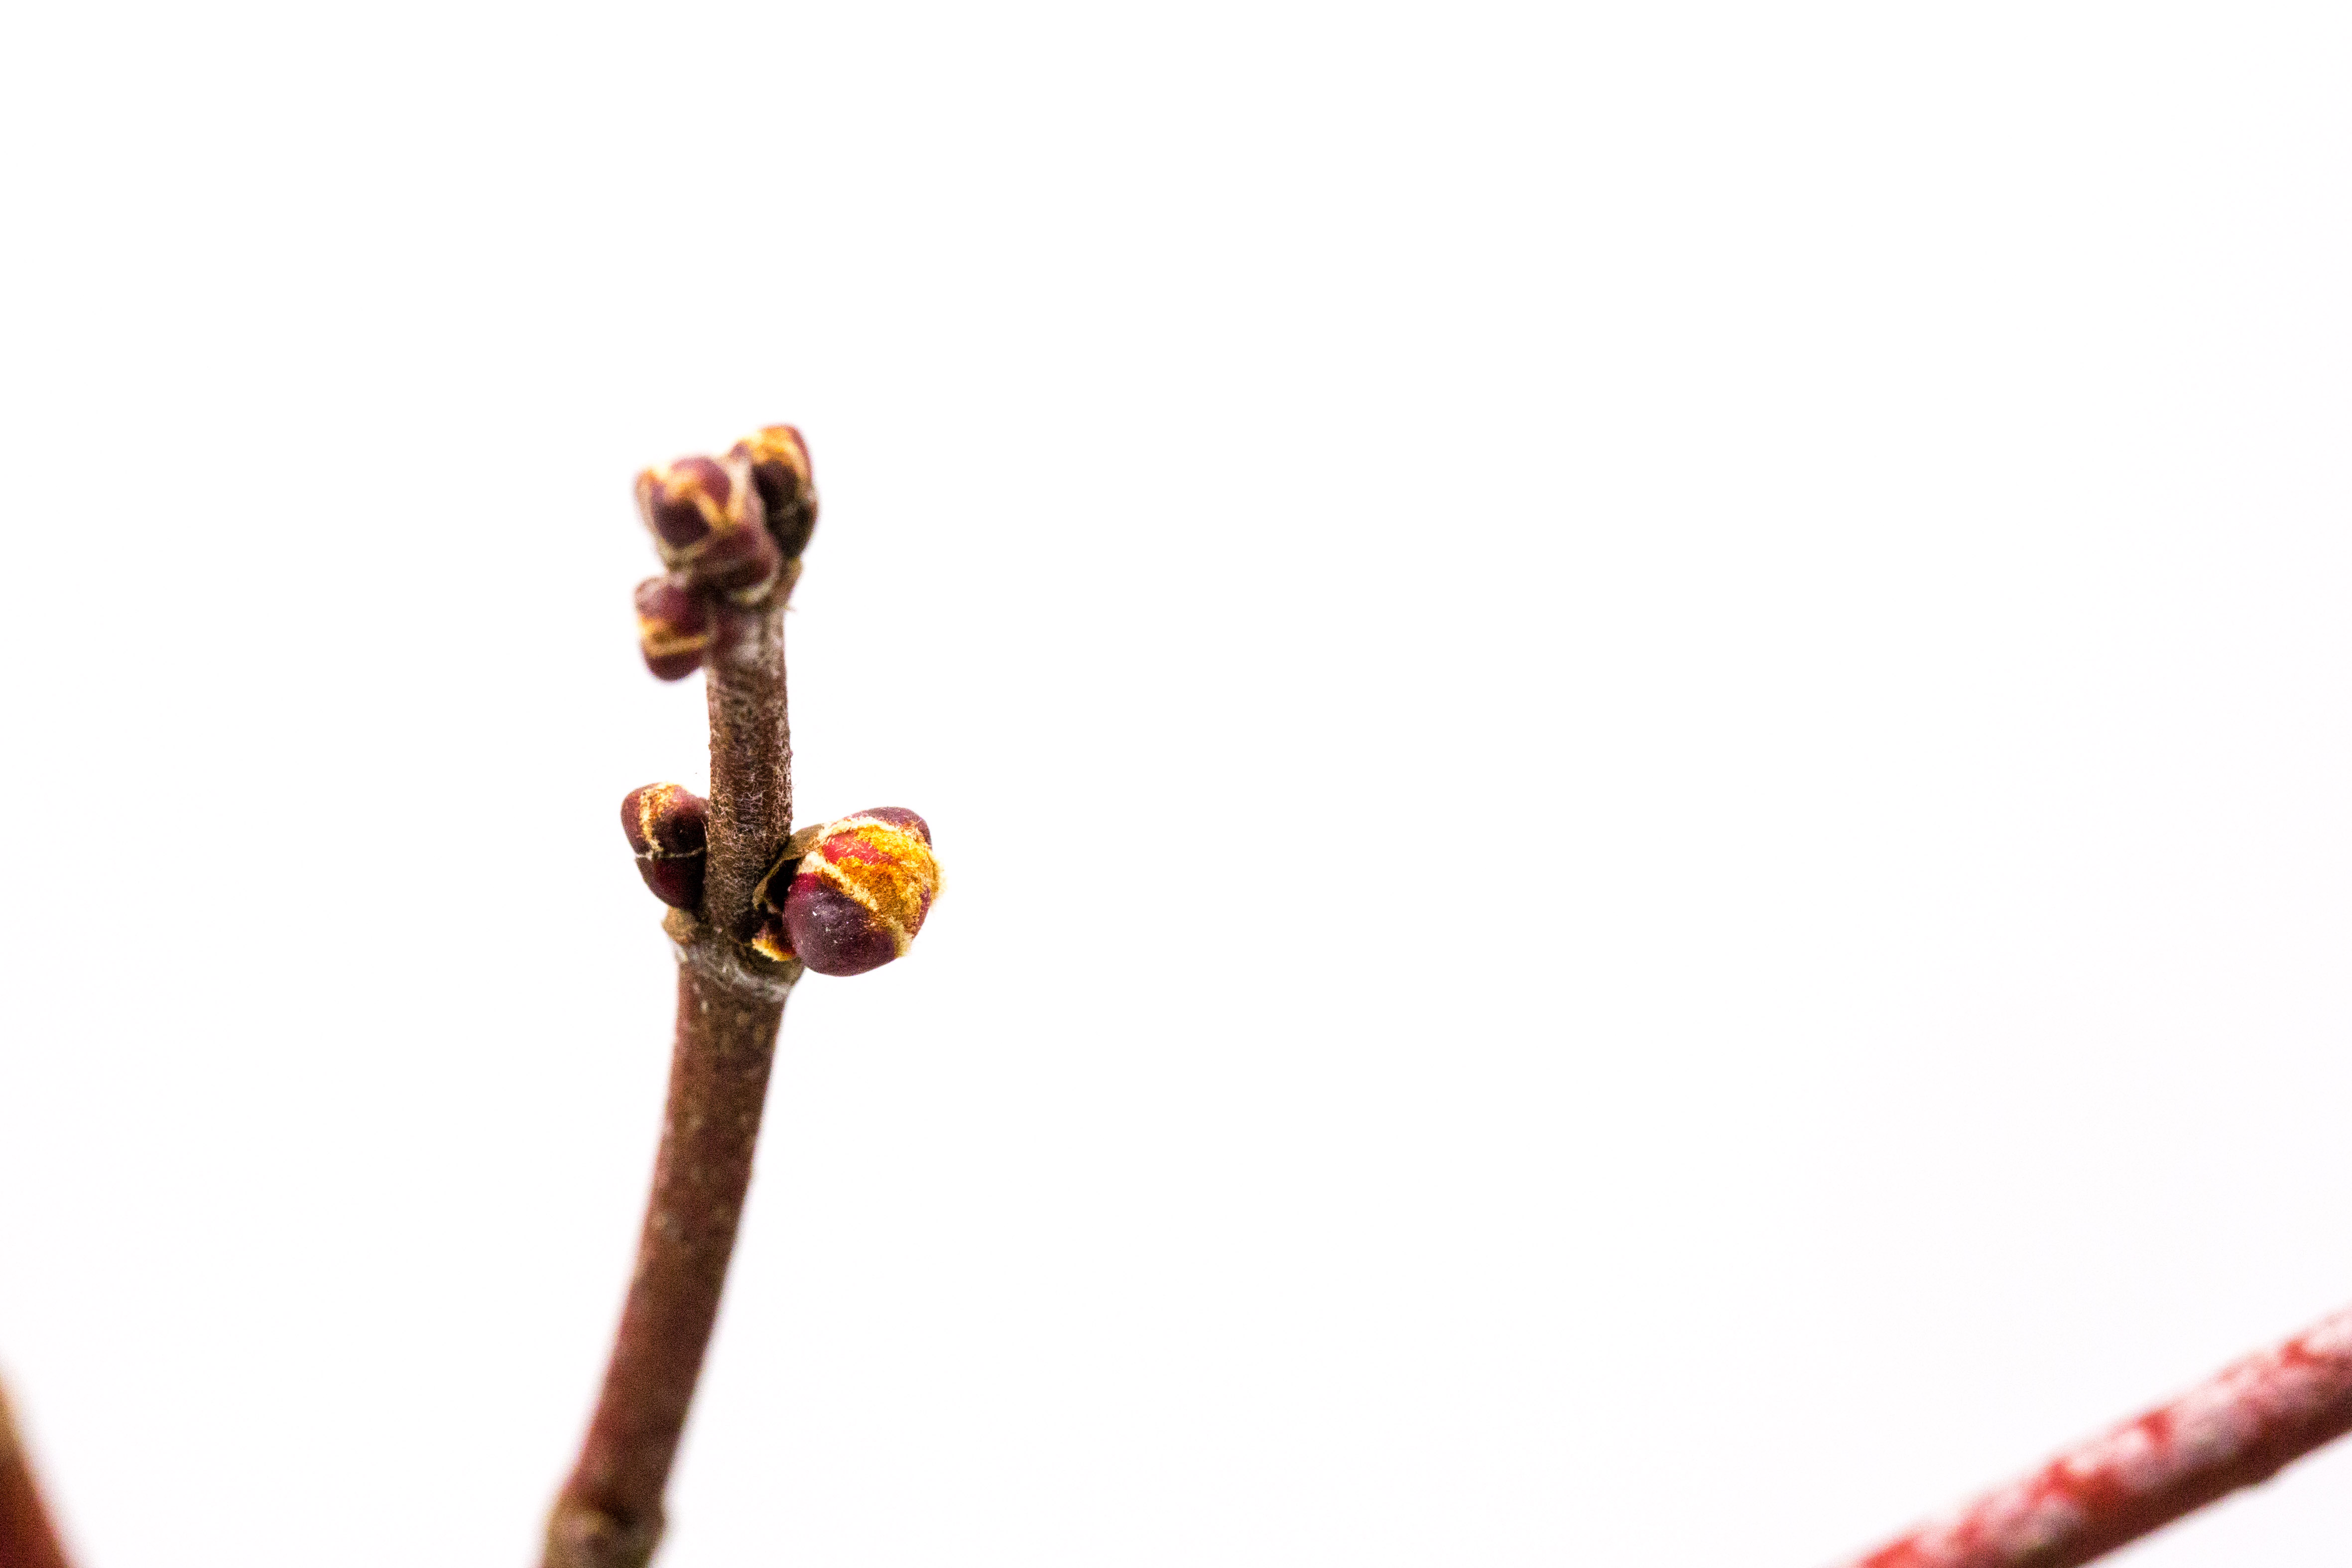
\includegraphics[width = 7cm]{acerub/Acer_rubrum,_stage_04.jpg}}
              \hfill \subfigure[Stage 5]{
                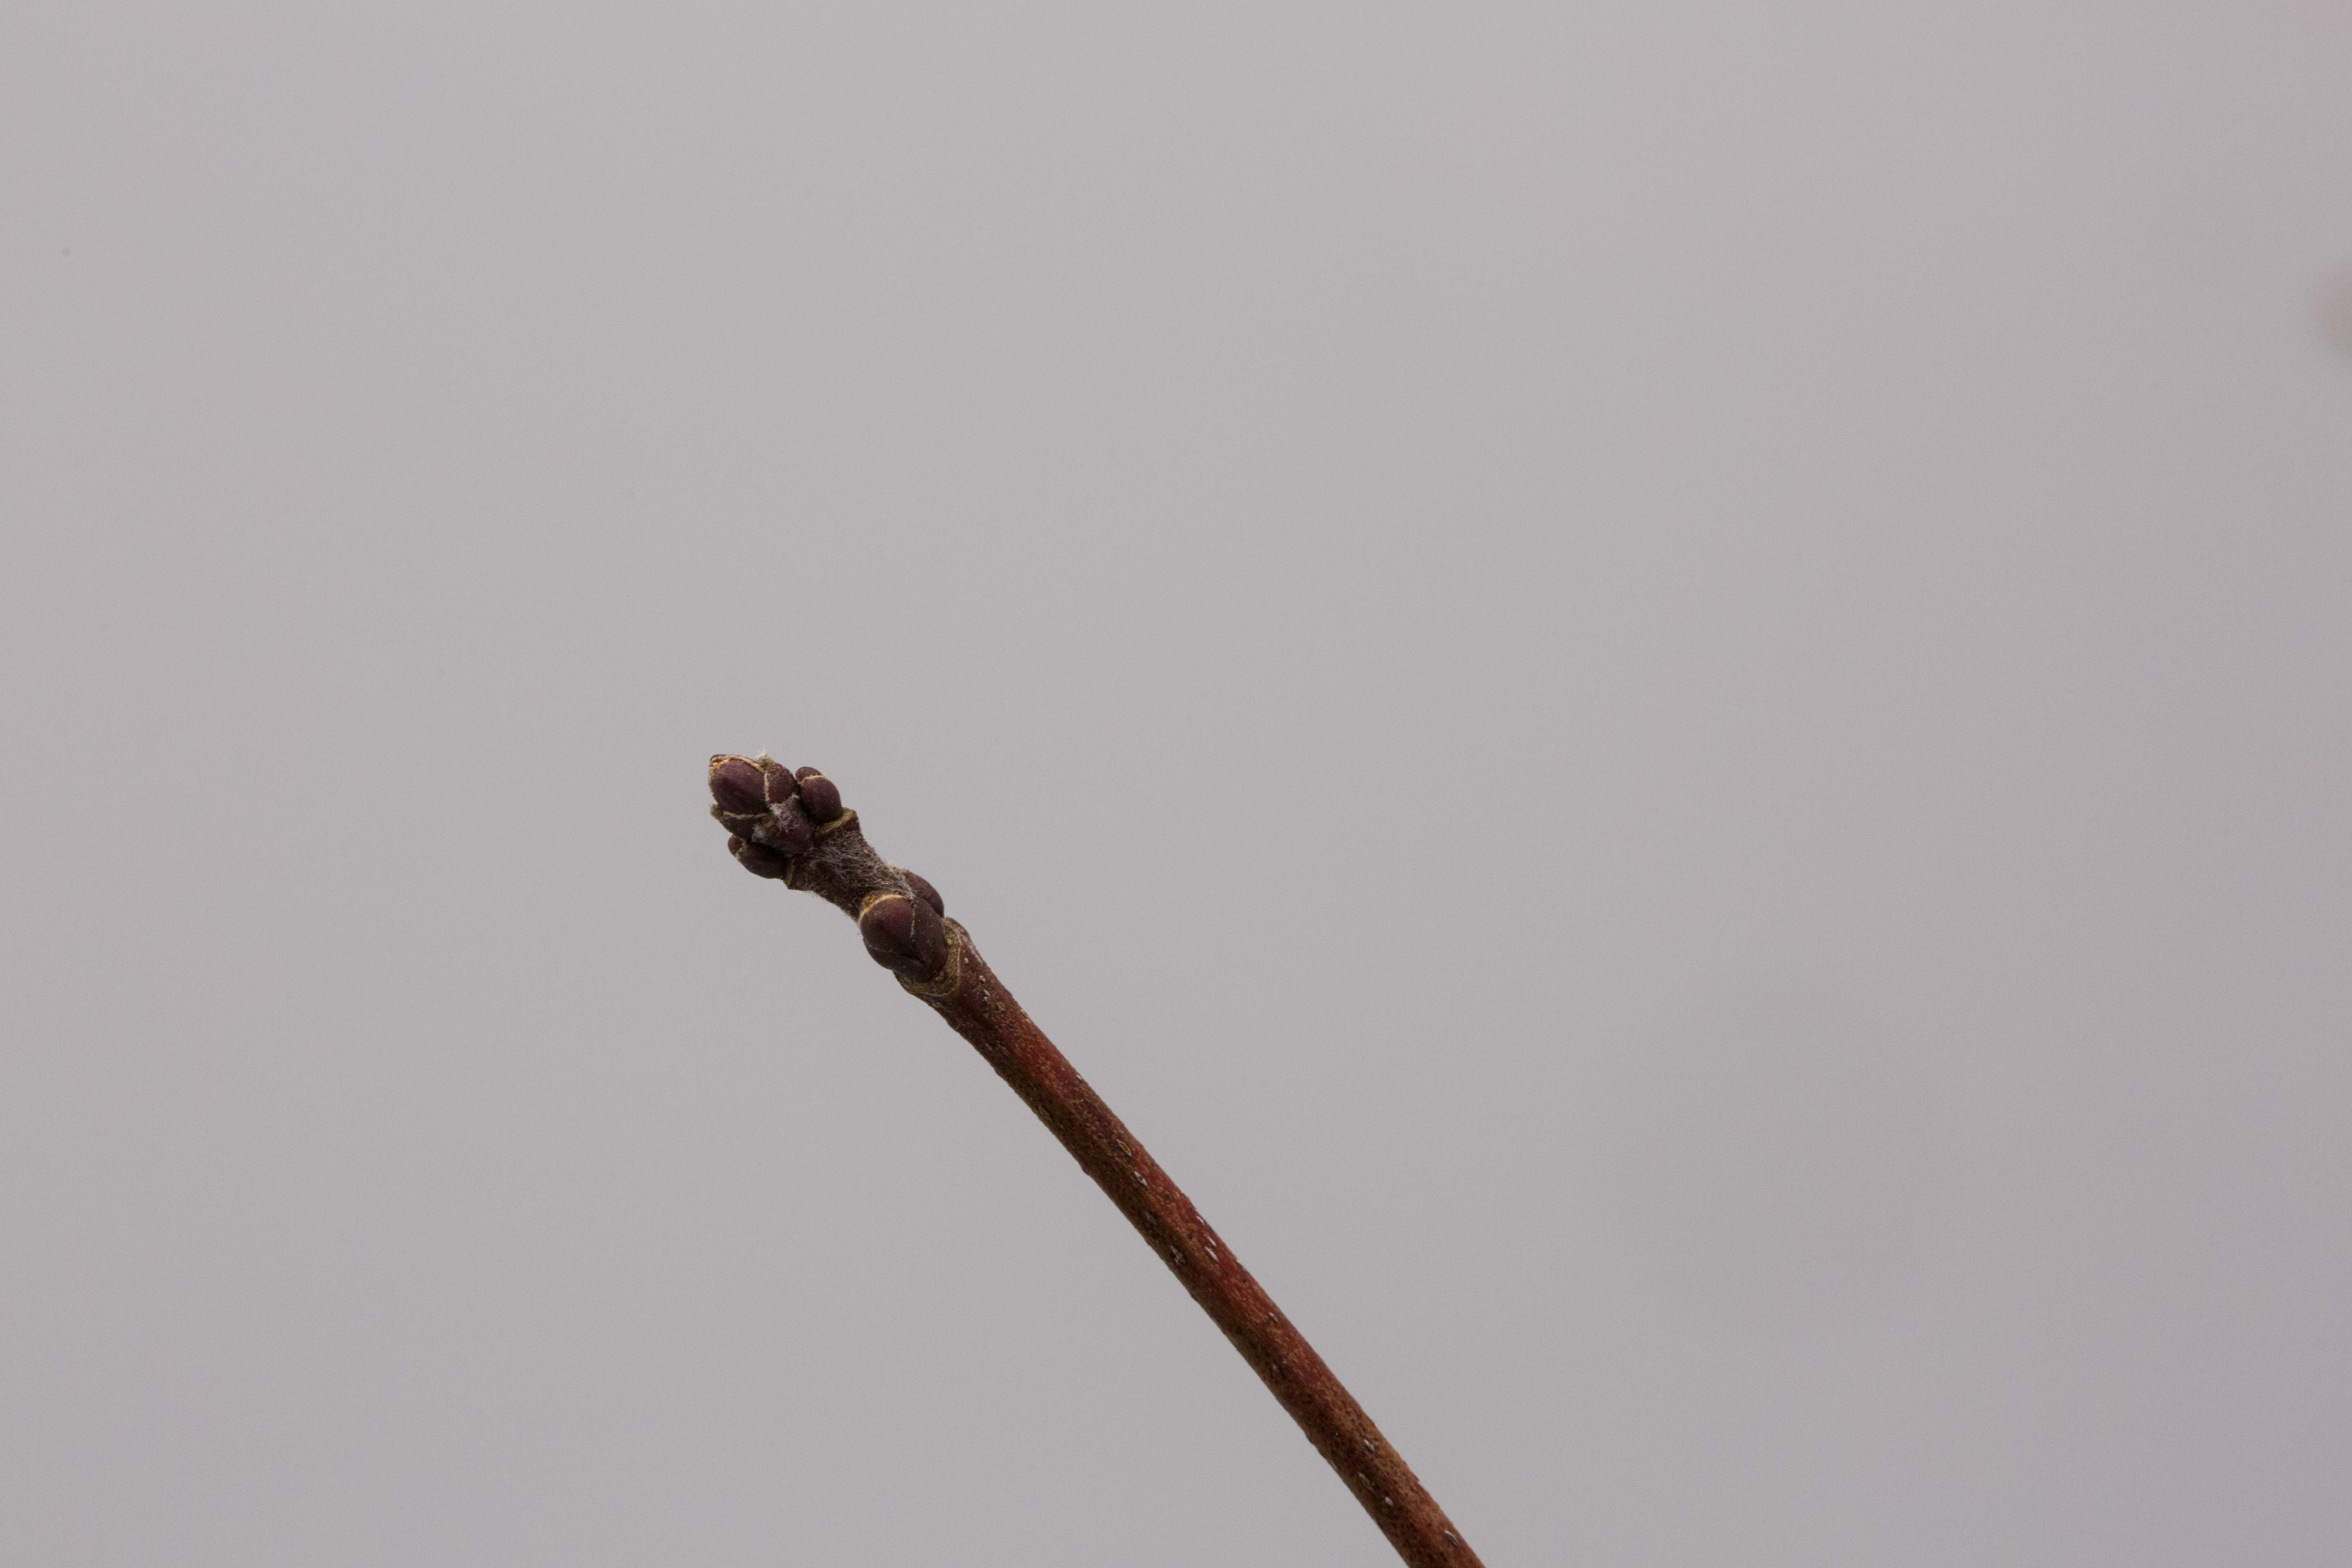
\includegraphics[width = 7cm]{acerub/Acer_rubrum,_stage_05.jpg}}
              \hfill \caption{\textit{Acer rubrum}}\end{figure}\newpage

%%%%%%%%%%%%%%%%%%%%%%%%%%%%%%%%%%%%
\section*{References Cited}
%%%%%%%%%%%%%%%%%%%%%%%%%%%%%%%%%%%%

\bibliography{BBCH}
\bibliographystyle{naturemag}

\end{document}
